\setcounter{rownumber}{0}
\chapter{Manuscript I: Laser cooling of traveling wave phonons in an optical fiber}
\label{ch:Cooling}
\acresetall

\textit{This chapter elaborates on experiments and results related to optomechanical cooling, which have been published as an article of the same name in Physical Review Applied by Johnson et al. (2023) \cite{johnson2023laser}. Any discrepancies, omissions, or errors that may exist between the published paper and this dissertation chapter are the sole responsibility of the author, as the text, analyses, and interpretations herein represent an independent and original presentation of the work.}

%--------------------------------------------------------------------%

\section{Introduction}
\label{sec:Cooling:Introduction}

Materials above the ground state experience therodynamic variations such as temperature and density. These thermal fluctuations alter the optical properties of a given material, allowing a scattering process to occur (see Section \ref{sec:Introduction:Light-Scattering}). Spontaneous Brillouin scattering is the inelastic scattering of light with these thermal fluctuations within a material, facilitating an energy exchange between the optical and acoustic domains. While a given medium typically supports a multitude of thermally excited acoustic modes (including both transverse and longitudinal modes) we focus here specifically on longitudinally travelling acoustic waves to demonstrate cooling in a continuous (non-resonant) system.

[lit review, state of the art]

%--------------------------------------------------------------------%

\section{Optomechanical Cooling and Heating}
\label{sec:Cooling:Cooling-Heating}

Backward Brillouin scattering targets longitudinally traveling acoustic waves (or phonons) through two complementary processes---Stokes and anti-Stokes, illustrated in Figures \ref{fig:Cooling:StokesHeating} and \ref{fig:Cooling:anti-StokesCooling}, respectively. In the Stokes process, an incident photon of frequency \(\omega\) scatters with a \textit{retreating} phonon of frequency \(\Omega\) annihilating the \textit{photon} and creating both an additional phonon of frequency \(\Omega\) and a backscattered photon at the difference energy (\(\omega_{\mathrm{Stokes}} = \omega - \Omega\)). In this way, both energy and momentum are conserved. This can be visualized by an analogy, in which the incident light experiences a doppler \textit{down}-shift in frequeny as though the photon were reflected from a retreating mirror. Since this processes results in an increase in the phonon population within the respective longitudinal mode of the material, this process is referred to as optomechanical heating. The energy lost by the light is gained by the material in the form of mechanical vibrations.

\begin{figure}[t]
    \centering
    \begin{subfigure}[b]{0.49\textwidth}
        \centering
        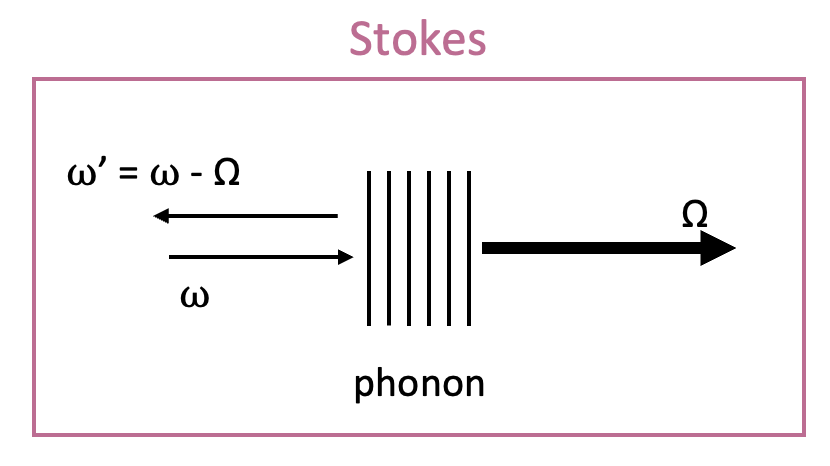
\includegraphics[width=\textwidth]{figs/3-Cooling/StokesHeatingProcess.png}
        \caption{}
        \label{fig:Cooling:StokesHeating}
    \end{subfigure}
    \hfill
    \begin{subfigure}[b]{0.49\textwidth}
        \centering
        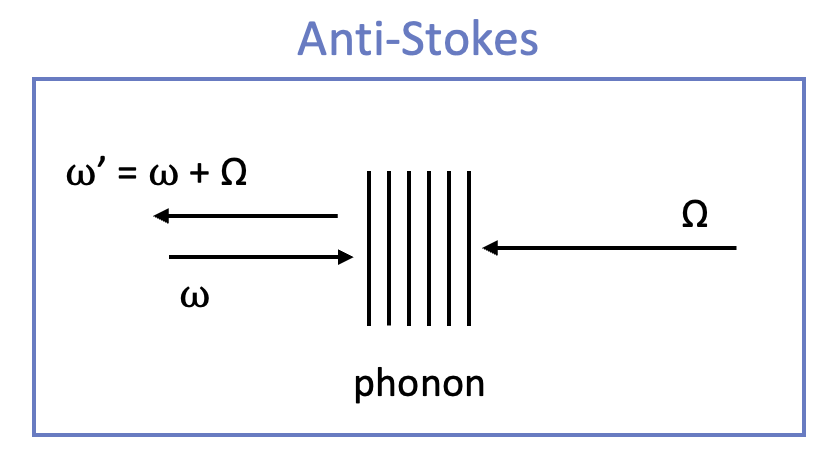
\includegraphics[width=\textwidth]{figs/3-Cooling/anti-StokesCoolingProcess.png}
        \caption{}
        \label{fig:Cooling:anti-StokesCooling}
    \end{subfigure}
    \caption{Illustration of optomechanical heating and cooling processes. Figure \ref{fig:Cooling:StokesHeating} shows an incident photon of frequency \(\omega\) scattering with a retreating phonon of frequency \(\Omega\), resulting in the annihilation of the incident photon and the creation of both an additional retreating phonon of frequency \(\Omega\) and a backwards propagating photon of reduced frequency and thereby energy (\(\omega_{\mathrm{Stokes}} = \omega - \Omega\)). Figure \ref{fig:Cooling:anti-StokesCooling} shows the inverse process, whereby an incident photon, \(\omega\), scatters with an approaching phonon, \(\Omega\), annihilating the incident photon and the phonon to produce a backwards propagating photon of increased frequency and thereby energy (\(\omega_{\mathrm{anti-Stokes}} = \omega + \Omega\)).}
    \label{fig:Cooling:StokesProcesses}
\end{figure}

The anti-Stokes process is the inverse process, whereby an \textit{approaching} phonon of frequency \(\Omega\) scatters with an incident photon of frequency \(\omega\), annihilating the \textit{phonon} and creating a backscattered photon at the addition energy (\(\omega_{\mathrm{anti-Stokes}} = \omega + \Omega\)). Both energy and momentum are again conserved, however in the anti-Stokes process, the incident light experiences a doppler \textit{up}-shift in frequency as if, to continue the analogy, the photon were reflected from an approaching mirror. For further intuition, one might consider an elastic collision of a ball (the photon) with a moving wall (the phonon) for the cases of the wall moving towards (in the anti-Stokes process) or away (in the Stokes process) from the ball as they collide. This simple analogy helps illustrate how momentum and energy are exchanged in optomechanical heating (Stokes) and cooling (anti-Stokes) processes.

While these processes naturally lead to a change in phonon population and thereby mode temperature, specific challenges arise in practical demonstration and detection of the phenomena. The most significant challenge is that since we are seeking to address the natural thermal phonons of the medium, we are restricted to a spontaneous Brillouin scattering regime as opposed to stimulated. Stimulated Brillouin scattering techniques are often employed to dramatically increase scattered power and aid in detection (see Appendix \ref{appendix:comparison} and specifically Figure \ref{fig:SponBSvsStimBSvsCoBS} for a comparison of scattered power produced by different Brillouin techniques). However, when stimulated conditions are met, the thermal phonons of the medium are actively driven, often by the injection of an additional optical field. Therefore, the stimulated scattering process is no longer a result of spontaneous thermal phonons but rather of optically driven phonon populations. As explained in Appendix \ref{appendix:comparison}, the condition for achieving stimulated Brillouin scattering is an overall process gain factor, \(G = G_{B}P_{P}L\), much greater than unity \((G \gg 1)\), where \(G_{B}\) is the effective Brillouin gain, \(P_{P}\) is the pump power, and \(L\) is the effective length. An ideal testbed for demonstrating optomechanical cooling would therefore feature an overall process gain factor near but not exceeding unity in order to maximize feasibility of measurement while ensuring a spontaneous scattering regime.

In addition to this fundamental requirement, rate conditions provide additional criticl constraints. The rate at which the phonons are depleted through the optomechanical cooling process must exceed the replenishment rate by the surrounding thermal bath.

Ideal testbed for demonstrating optomechanical cooling:

\begin{enumerate}
\item Large acousto-optic coupling
\item Tight confinement of light and sound
\item Sound speed not too fast (too large brillouin frequency shift, expensive fast elecronics for detection) or too slow (too small brillouin frequency shift, making it hard to separate sideband from carrier)
\item Large single pass gain GPL
\item Fast escape condition - phonon mode depletion rate must exceed repopulation rate \(4v_{g}/L \gg \Gamma\)
\end{enumerate}

%--------------------------------------------------------------------%

\section{Cooling Platform: \texorpdfstring{$CS_{2}$}{CS2}-Liquid Core Optical Fiber}
\label{sec:Cooling:Platform}

Demonstration of optomechanical cooling and heating of traveling wave phonons requires a device or material host that [can balance all of the requirements I just layed out in the previous section!] features large optomechanical coupling as well as tight optical and acoustic confinement for large acousto-optic overlap. A \ce{CS2}-filled \ac{LCOF} similar to that used by Behunin et al. (2019) was used.\cite{behunin2019spontaneous}


\section{Fabrication of \texorpdfstring{$CS_{2}$}{CS2}-Liquid Core Optical Fiber}
\label{subsec:Cooling:Platform:Fabrication}

\begin{figure}[t]
  \centering
  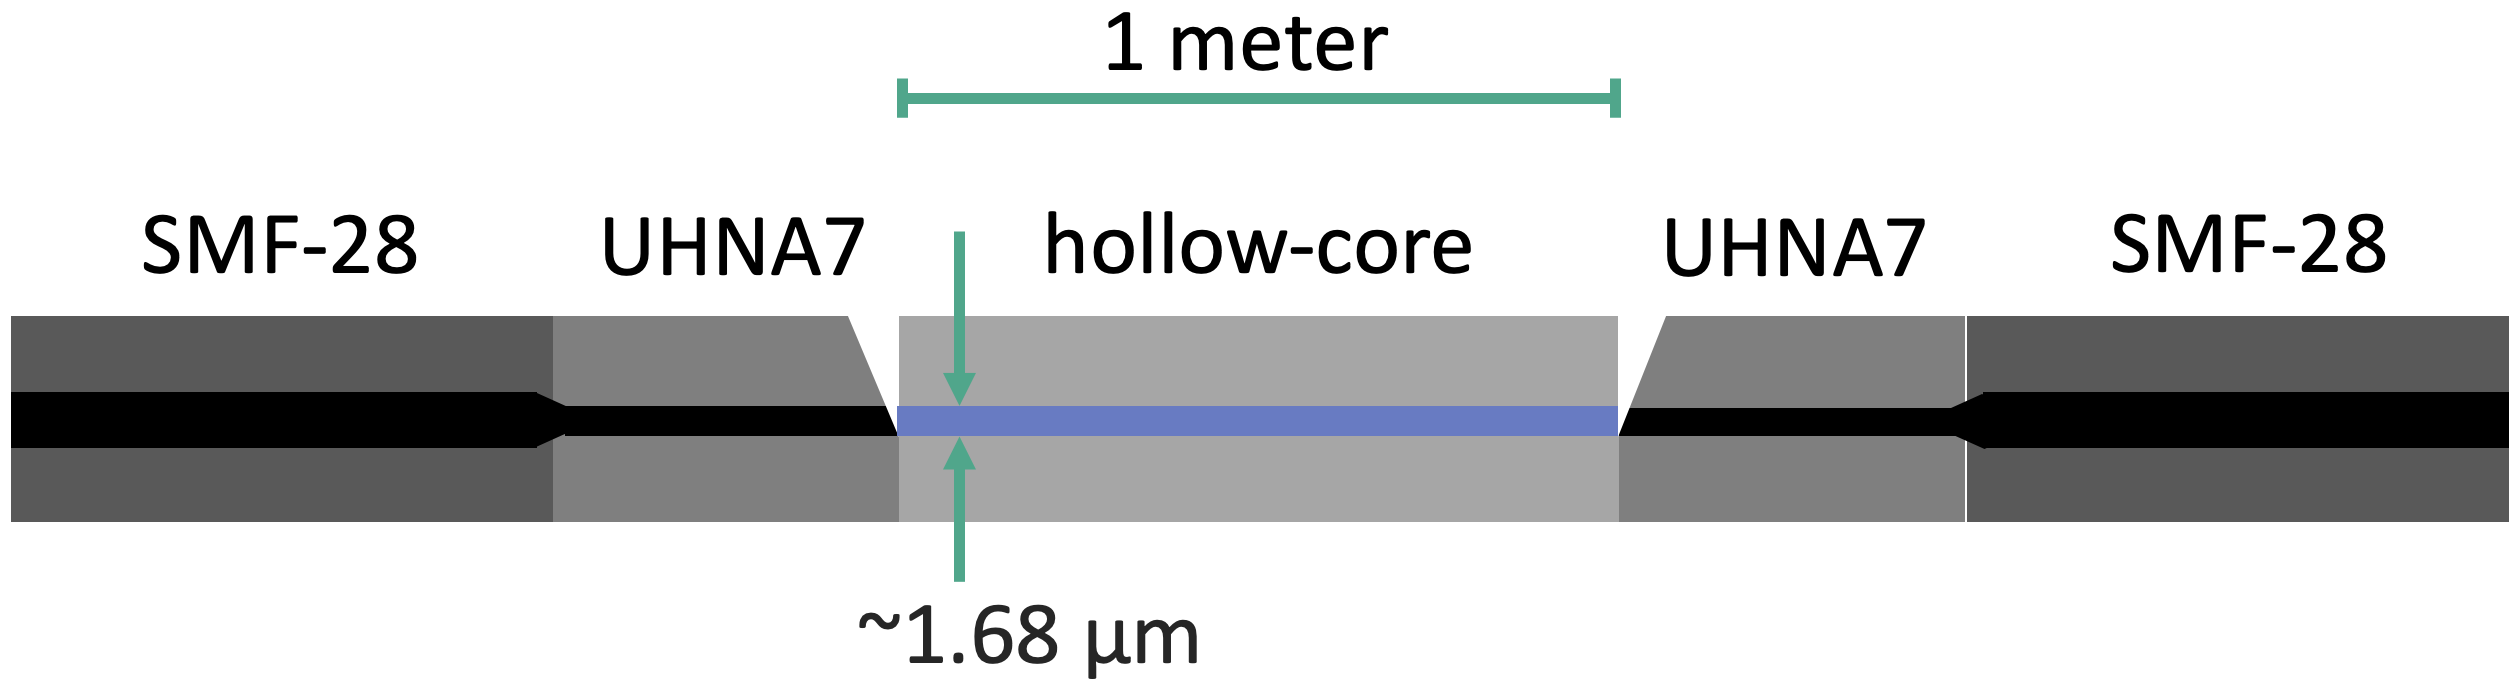
\includegraphics[width=\textwidth]{figs/3-Cooling/LCOFdiagram.png}
  \caption{Schematic of \ac{LCOF} design. A length of \ac{SMF-28} is arc-spliced to 5-\SI{10}{\centi\meter} of \ac{UHNA7} fiber, with a post-arc process applied to taper the larger \ac{SMF-28} core down to the smaller \ac{UHNA7} core for better mode matching and coupling efficiency. The \ac{UHNA7} fiber is angle-cleaved and fusion-spliced to a flat-cleaved hollow-core fiber via a heated filament in a Vytran fusion splicer system. The angle cleave results in a splice that only partially fuses the two fibers, leaving a pathway for liquid to enter the hollow core fiber via capillary action once submerged. A mirrored splice configuration on the other end of the length of hollow-core fiber allows air to escape as the fiber fills, and a reverse taper again provides improved mode matching for the light to recouple into \ac{SMF-28}.}
  \label{fig:LCOF diagram}
\end{figure}

The fabrication process for the \ce{CS2}-\ac{LCOF} involved several key steps for each of the two ends: splicing \ac{SMF-28} to \ac{UHNA7} fiber, preparing and angle-cleaving fibers, cutting and preparing a protective glass vial, and finally securing the assembly on a microscope slide. Figure \ref{} illustrates the overall schematic of the fiber fusion strategy, showing how \ac{SMF-28} and \ac{UHNA7} fibers flank the hollow core. The following sections detail each step in the fabrication protocol.

\subsection{Splicing \ac{SMF-28} to \ac{UHNA7}}

Before integrating the hollow-core segment, a segment of Corning \ac{SMF-28} was spliced to Thorlabs \ac{UHNA7} fiber. This transition was necessary to gradually match the mode fields and reduce losses at the interface with the hollow-core region.

To begin, a short length (\SI{0.5}{\meter}) of \ac{SMF-28} was stripped, cleaved flat, and arc-spliced to 5–\SI{10}{\centi\meter} of similarly prepared \ac{UHNA7} fiber. The \ac{UHNA7} fiber was fully stripped of its coating prior to arc-splicing. This was done to prevent up-and-down bending of the fiber end in subsequent horizontal alignment with the Vytran fusion splicer. The initial splice was performed with standard parameters, but the arc was then repeated four to five times in order to produce a “tapering” effect which helped narrow the \ac{SMF-28} core (\SI{9.2}{\micro\meter} diameter) where it contacted the smaller \ac{UHNA7} core (\SI{2.4}{\micro\meter} diameter), improving coupling efficiency. Prior to and following the splice, optical transmission measurements were taken to assess the splice quality and ensure maximum transmission was preserved.

\subsection{Preparing the \ac{UHNA7} Fiber}

After the preliminary \ac{SMF-28}–\ac{UHNA7} splice, the \ac{UHNA7} fiber needed to be angle-cleaved to ensure a gap remained for \ce{CS2} to be able to enter the hollow-core fiber after fusion-splicing the two fiber segments. An angle-cleaver with an adjustable torque and tension mechanism was used for this process. The angle-cleaved \ac{SMF-28}-\ac{UHNA7} segment was then loaded into the Vytran fusion splicing system:

\begin{enumerate}
	\item Equipment Setup: The Vytran fusion splicing station and its vacuum pump were turned on, and the system’s dedicated software interface was opened. Approximately two minutes was allowed for the vacuum level to stabilize.
	\item Fiber Positioning: The left fiber clamp block was pivoted fully to the left, and the \ac{UHNA7} fiber was placed so that its freshly cleaved tip was centered over the reference circle at the splice head.
	\item Alignment: While the vacuum held the fiber in place, the system’s camera view was used to rotate the fiber such that the sharpest angle of the \ac{UHNA7}’s end face was in the camera's view. A small “flag”—a piece of unstripped fiber with a small tape handle on one end—was used as needed to help the clamp grip the bare \ac{UHNA7} fiber securely.
	\item Pivot and Support: The left block was pivoted back and forth until the \ac{UHNA7} tip was near the correct horizontal position. A folded piece of support paper and two boxes of Kimtech Kimwipes on the benchtop were used to prevent the fiber from drooping and to minimize the risk of breakage during handling.
\end{enumerate}

\begin{figure}[t]
  \centering
  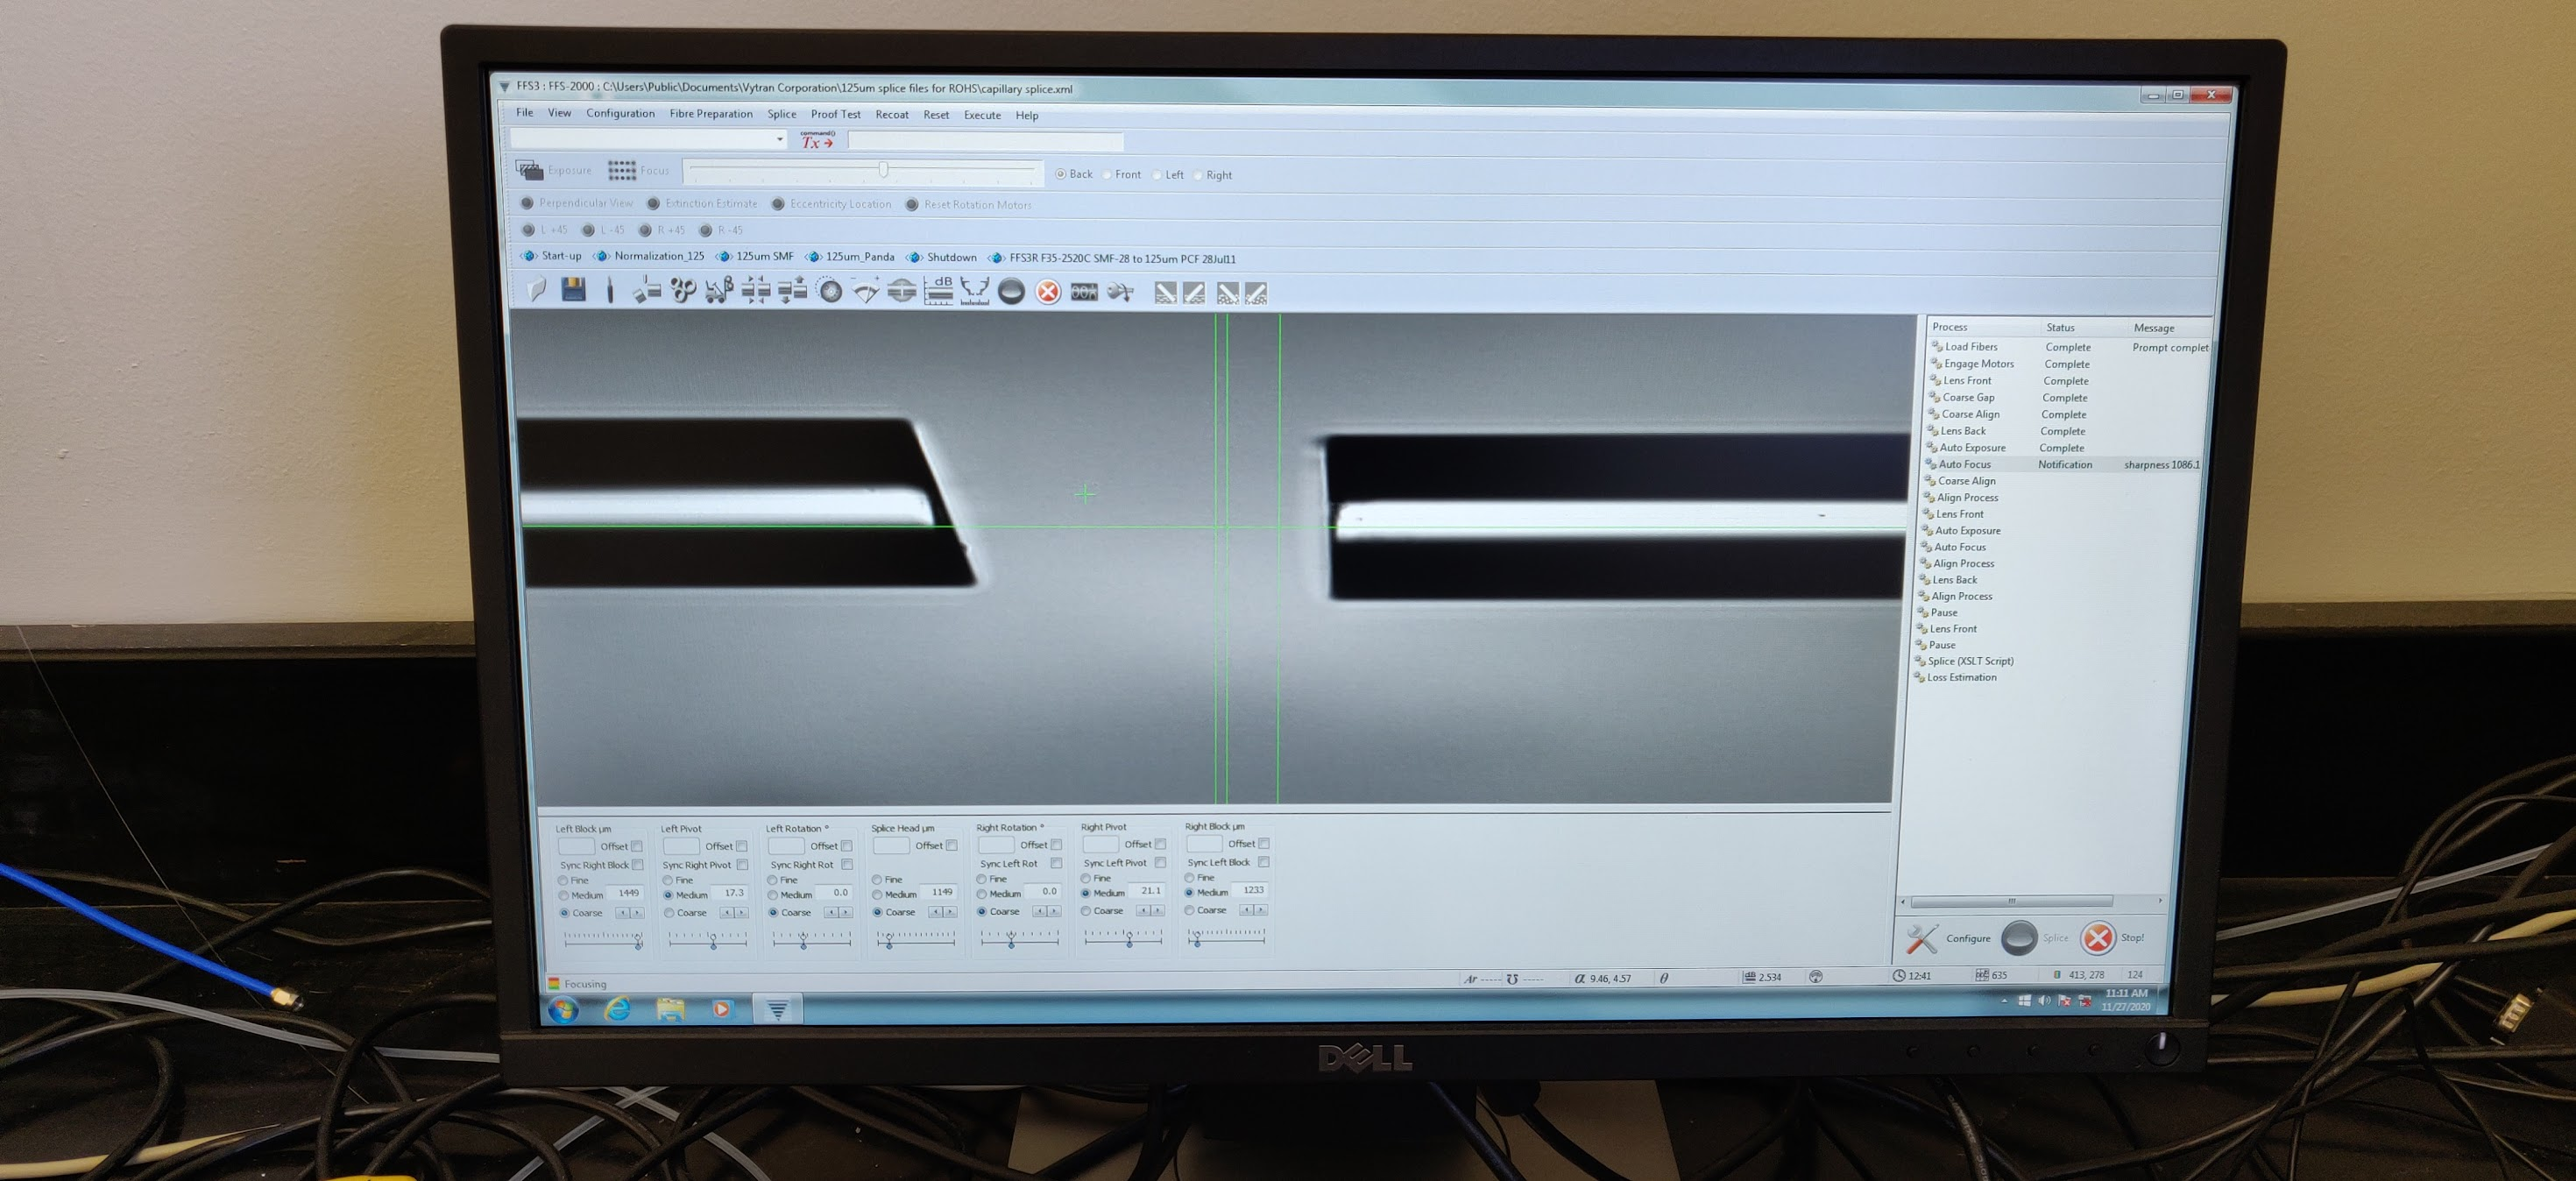
\includegraphics[width=\textwidth]{figs/3-Cooling/vytranCameraPreSplice.jpg}
  \caption{Picture of Vytran software interface camera imaging system showing a microscope view of the two fiber ends pre-splice (Section~\ref{subsec:Cooling:Fusion-Splicing to Hollow-Core}). The left angle-cleaved fiber is the \ac{UHNA7} fiber. The right flat-cleaved fiber is the hollow-core fiber. Subsequent alignment processes, first automatic then manual fine-tuning, align the fibers in xy space for optimal fusion-splicing and optical transmission once filled.}
  \label{fig:vytran camera pre splice}
\end{figure}

\subsection{Preparing the Hollow-Core Fiber}

Once the \ac{UHNA7} fiber was properly angle-cleaved, the hollow-core fiber segment was prepared for splicing:

\begin{enumerate}
	\item Stripping and Cleaving: The hollow-core fiber coating was gently dissolved in acetone and wiped away to expose the bare glass. It was then cleaved flat rather than at an angle.
	\item Positioning on the Vytran fusion splicer: The right clamp block was pivoted to its stop position, and the hollow-core fiber was placed so its end was centered over the splice head’s circle, ensuring no physical contact with the \ac{UHNA7} fiber.
	\item Flag and Alignment: As with the \ac{UHNA7}, a flag of unstripped fiber was placed above the hollow-core fiber to facilitate stable clamping. The right clamp block was slowly pivoted toward the center until the fiber tips were close but still not touching. Like before, the fiber was supported with folded paper and Kimwipe boxes to prevent bending.
\end{enumerate}

\begin{figure}[t]
  \centering
  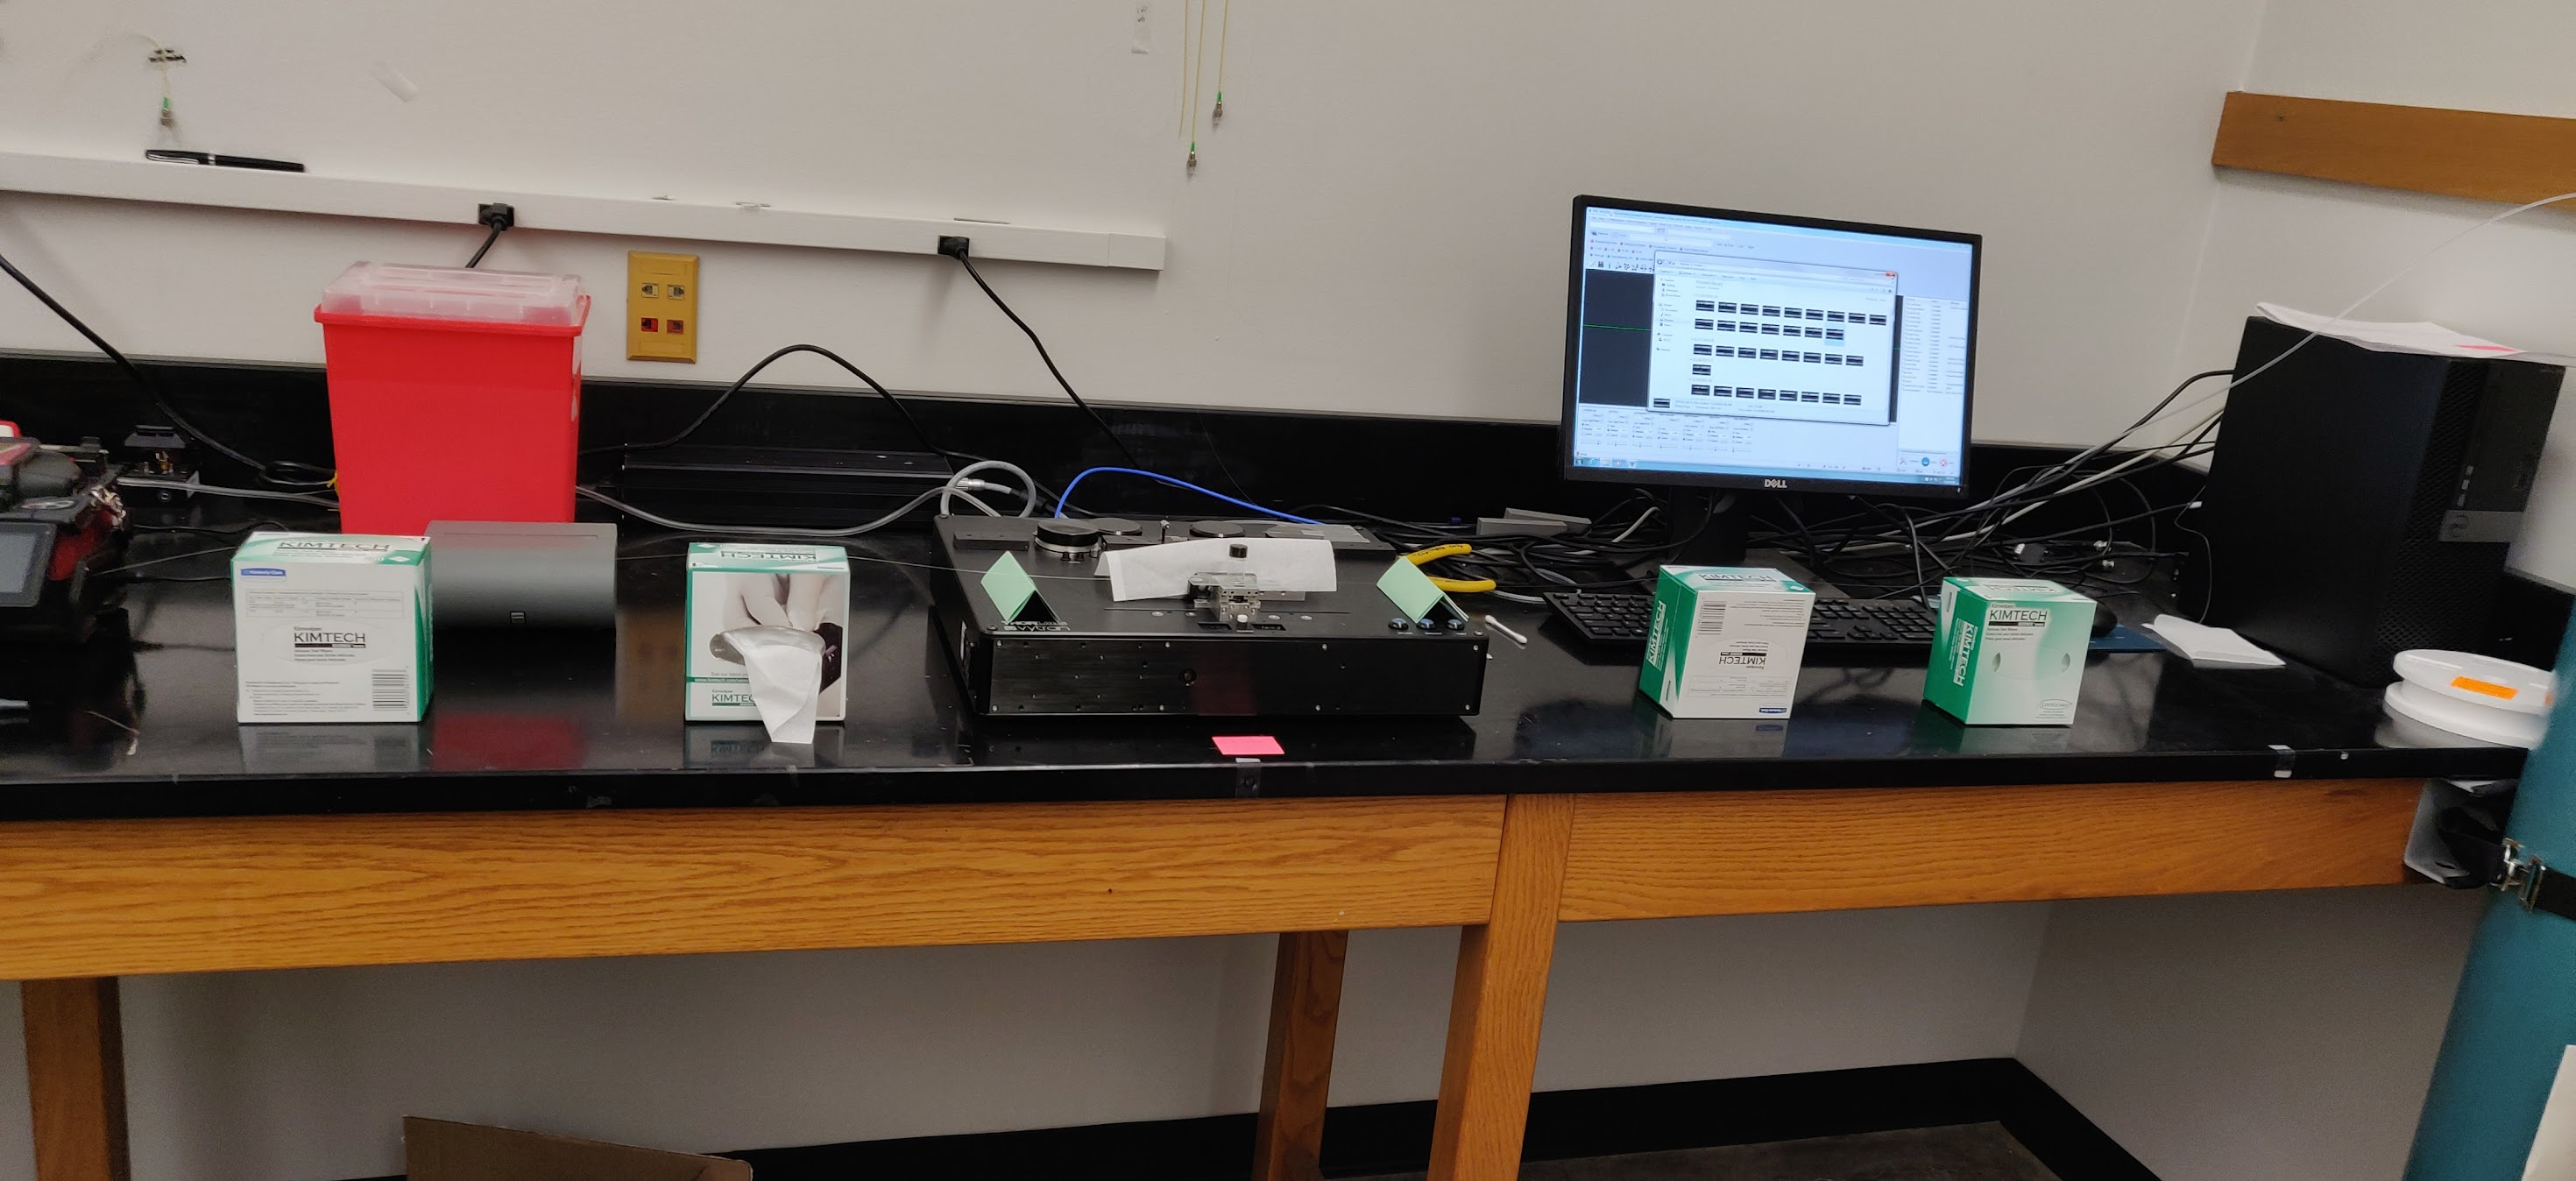
\includegraphics[width=\textwidth]{figs/3-Cooling/doubleBoxBracedSplice.jpg}
  \caption{Picture of both lengths of fiber braced by folded paper and two Kimwipe boxes on either side to prevent bending and flexing while transferring the delicate splice onto a glass slide (Section~\ref{subsec:Cooling:Transferring the Spliced Fibers onto the Slide}).}
  \label{fig:double box braced splice}
\end{figure}

\subsection{Cleaning and Preparing the Microscope Slide}

Because the final splice assembly must be encapsulated for protection, it was mounted on a clean microscope slide. The slide was scrubbed with soap and a soft toothbrush under running hot water, then thoroughly rinsed and dried with an air gun. Clean handling was crucial, so the slide was placed inside a folded Kimwipe for safekeeping until needed.

\subsection{Cutting and Preparing the Glass Vial}

A small glass vial was used to form a protective enclosure over the splice region and allow liquid to fill the hollow core.

\begin{enumerate}
	\item Cutting the Vial: Wearing gloves and safety glasses, a new glass vial was secured carefully by hand and cut at low rotational speed on a saw. The cut removed only the bottom portion of the vial so that the main body of the vial remained relatively long.
	\item Flattening and Notching: The cut edge was smoothed and flattened with a file block, and two shallow, wide straddle-gaps were added on opposite sides of the new opening. These gaps would later accommodate the fiber on the slide.
	\item Cleaning: Finally, the vial was scrubbed with dish soap and a pipe cleaner, rinsed, dried with compressed air, and recapped until needed.
\end{enumerate}

\begin{figure}[t]
    \centering
    \begin{subfigure}[b]{\textwidth}
        \centering
        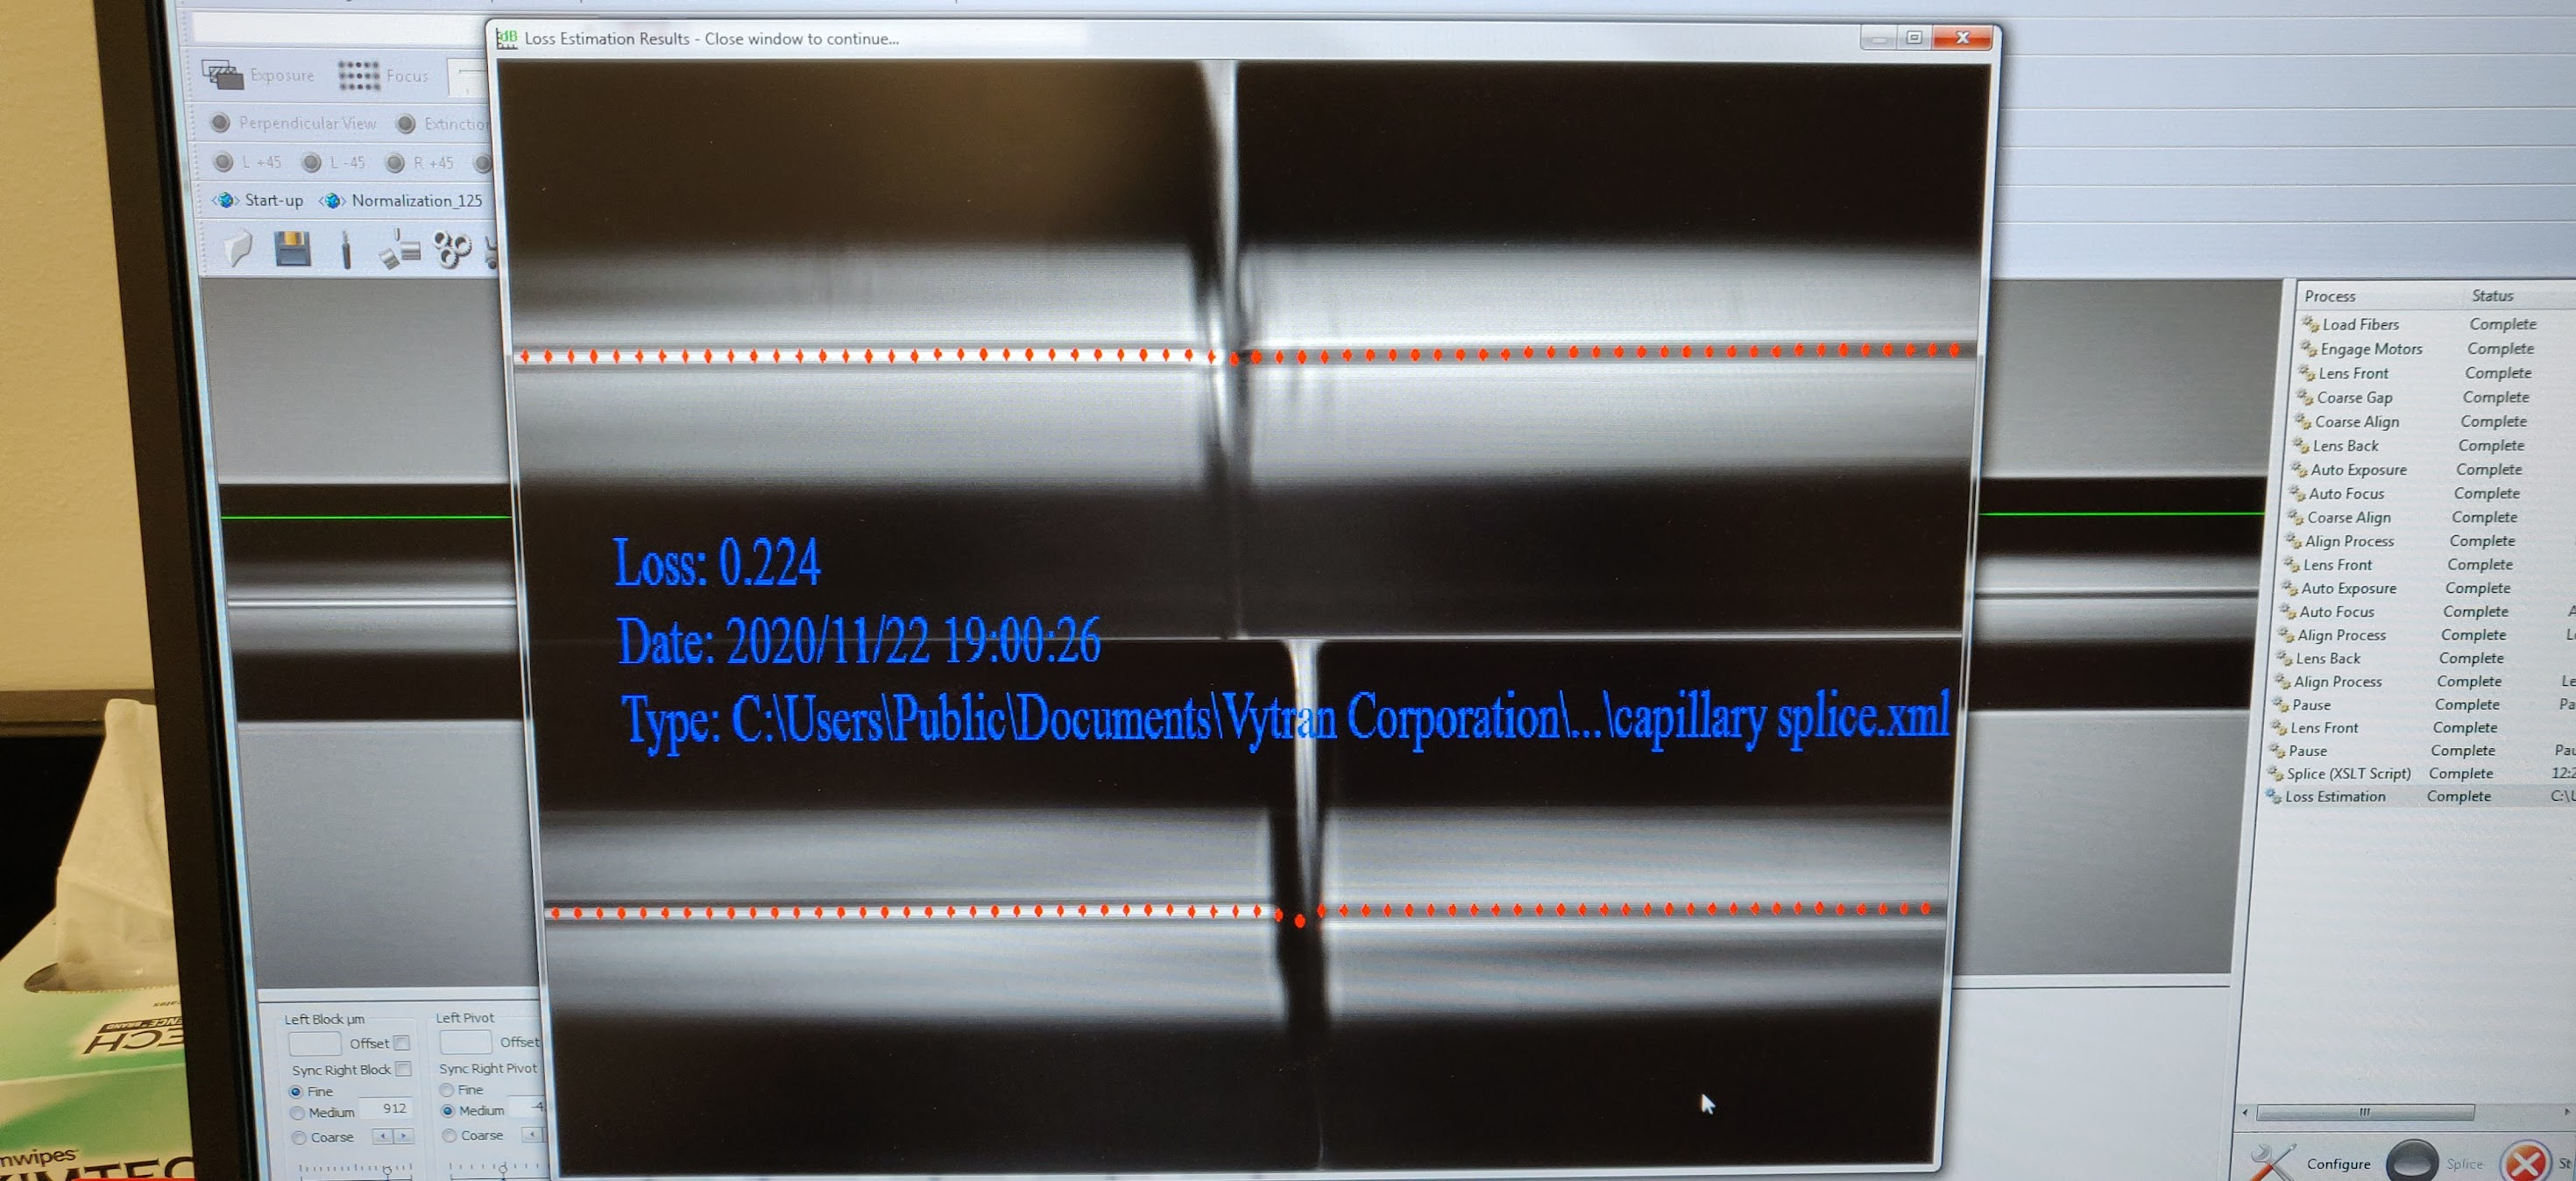
\includegraphics[width=\textwidth]{figs/3-Cooling/bigGapSplice.jpg}
        \caption{}
        \label{fig:Cooling:big gap splice}
    \end{subfigure}
    \vspace{0.5cm}
    \begin{subfigure}[b]{\textwidth}
        \centering
        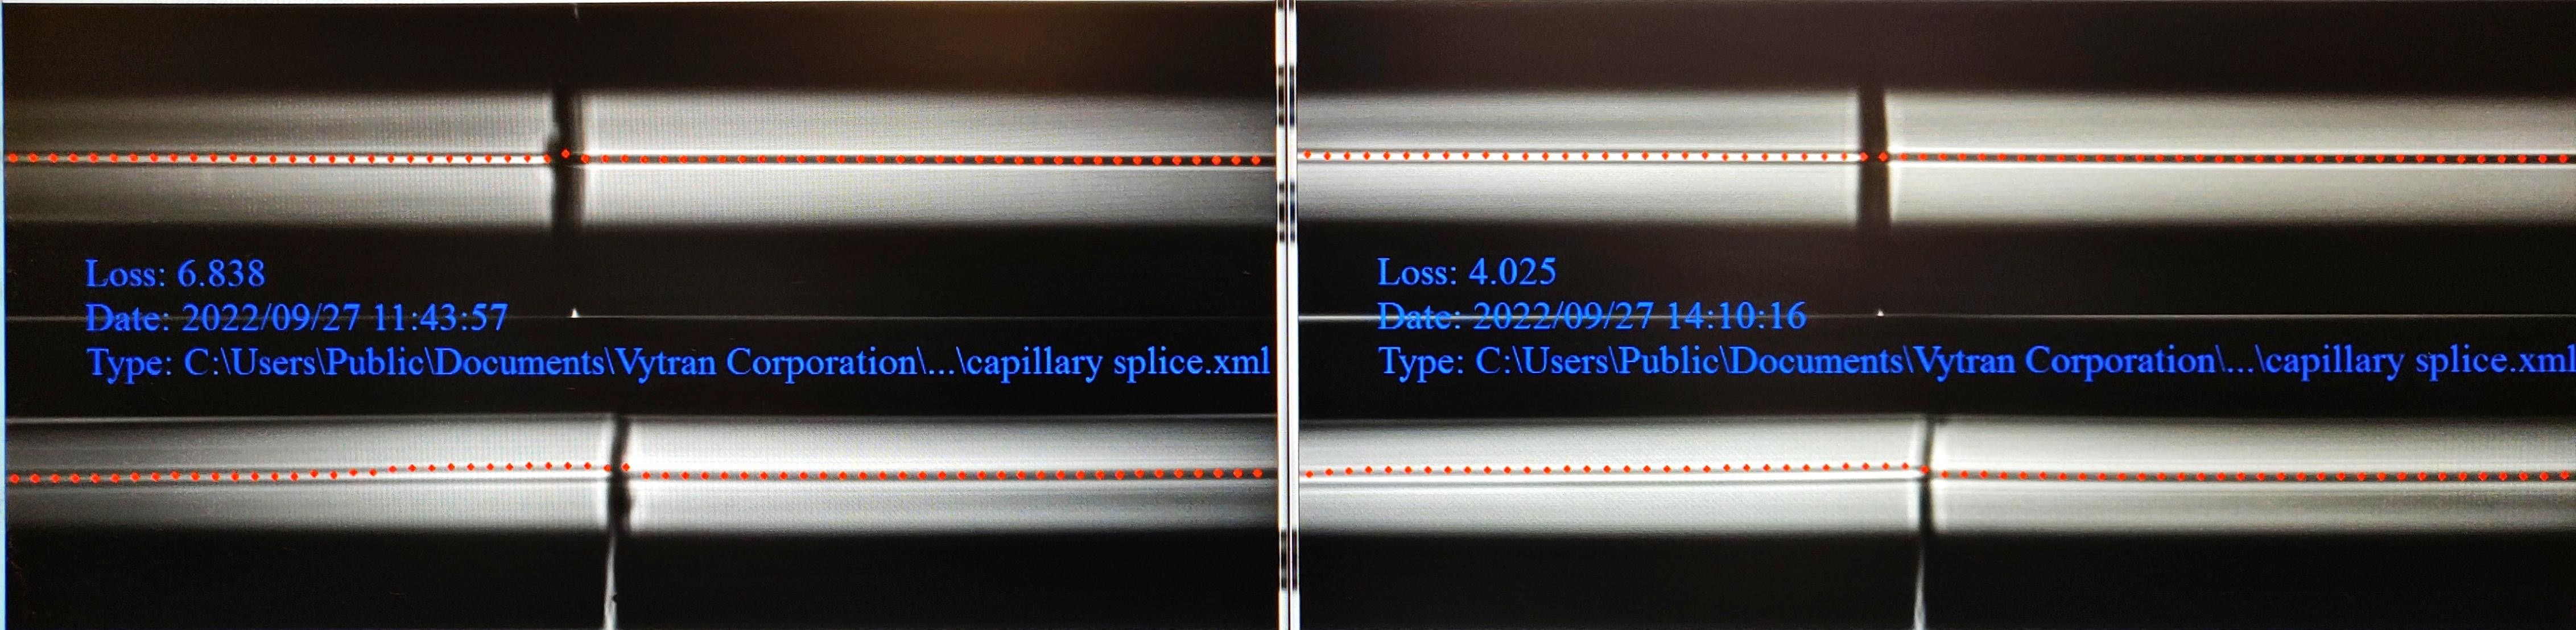
\includegraphics[width=\textwidth]{figs/3-Cooling/finalSampleVytranSplice.jpeg}
        \caption{}
        \label{fig:Cooling:final splice used for data}
    \end{subfigure}
    \caption{Example images of \ac{LCOF} splices (Section~\ref{subsec:Cooling:Fusion-Splicing to Hollow-Core}). Figure (a) shows an earlier example of a splice which featured a large visible wedge-shaped gap for liquid to enter the hollow-core fiber. While gaps of this size were sometimes successfully transferred onto a slide, further investigation showed gaps of this scale to reduce optical transmission through the splice. This fact became critical later for collecting the data for the pump-probe experiment. Figure (b) shows images of the two splices featured on the ultimate sample which was used to gather final data for publication.}
    \label{fig:Cooling:example splice images}
\end{figure}

\FloatBarrier

\subsection{Fusion-Splicing the \ac{UHNA7} to the Hollow-Core Fiber}
\label{subsec:Cooling:Fusion-Splicing to Hollow-Core}

The next step was to form the final fusion splice between the \ac{UHNA7} fiber and the hollow-core segment within the fusion splicer:

\begin{enumerate}
	\item Positioning and Auto-Alignment: With both fibers supported and extending naturally from opposite blocks, the splicer’s auto-alignment was initiated. The system brought the fibers within viewing distance so the operator could adjust vertical and horizontal positioning.
	\item Core Alignment: Using the splicer’s camera interface, the UHNA7 core was lined up with the hollow-core’s central region. Small vertical and horizontal translations ensured good overlap.
	\item Fiber Touch-Off: The left fiber (\ac{UHNA7} side) was carefully advanced until the tips touched, then retracted two clicks for optimal separation during splicing. Precise final positioning of the fiber ends ensured that a small gap remained in the hollow core to accommodate liquid infiltration during the filling process. Simultaneously, this same fiber end positioning ensured the cladding regions were fused sufficiently to preserve splice integrity under the delicate handling steps that followed.
	\item Argon Gas Flow and Fusion: An argon flow was introduced to shield the fusion region from contaminants, and the fusion filament heating was applied. Images were taken at each step to verify the splice quality. If alignment or splicing was inadequate, the fibers were separated, re-cleaved if necessary, and the procedure repeated. After confirming a good splice, the argon was turned off and the splicer was shut down.
\end{enumerate}

\begin{figure}[t]
  \centering
  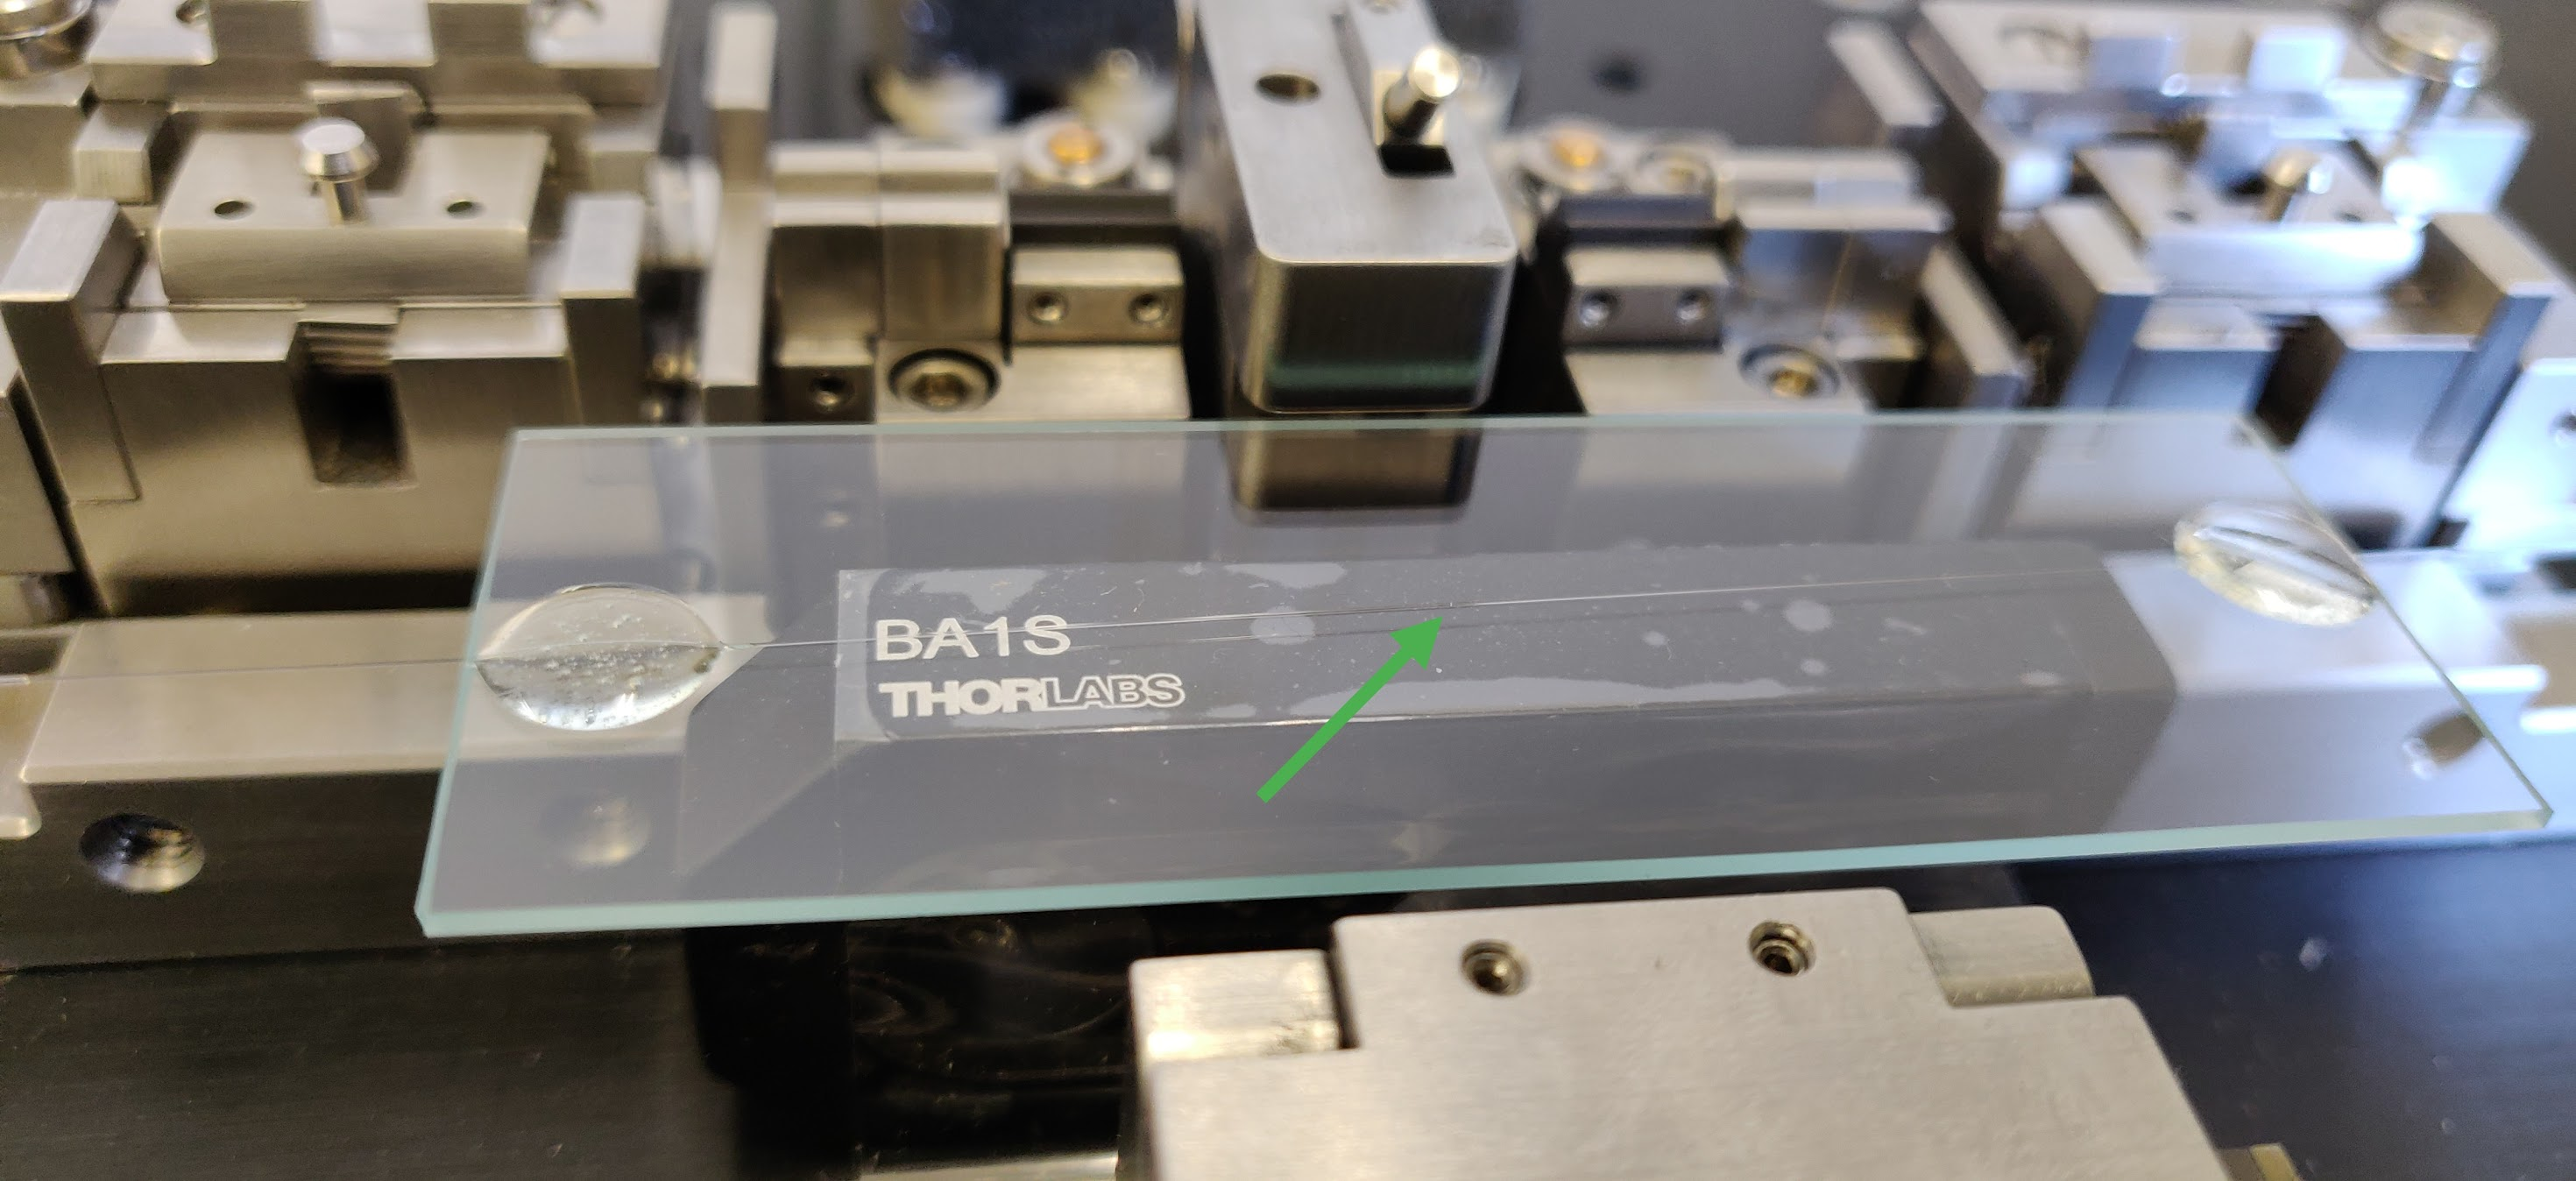
\includegraphics[width=\textwidth]{figs/3-Cooling/tackedSpliceWithArrow.jpg}
  \caption{Picture of splice successfully transferred onto a glass slide and tacked on either side with drops of epoxy (Section~\ref{subsec:Cooling:Transferring the Spliced Fibers onto the Slide}). An arrow points to the location of the critical splice between the angle-cleaved \ac{UHNA7} fiber and the flat-cleaved hollow-core fiber.}
  \label{fig:tacked splice with arrow}
\end{figure}

\subsection{Transferring the Spliced Fibers onto the Slide}
\label{subsec:Cooling:Transferring the Spliced Fibers onto the Slide}

Upon completing the angle splice, the fiber assembly needed to be moved gently off the splicer onto the prepared microscope slide:

\begin{enumerate}
	\item Release and Stabilization: With the splicer’s vacuum pump still on to hold the splice securely, the magnetic latches clamping the fiber on either side of the splice to the translation/rotation stages were carefully lifted. Tweezers were used to remove any fiber “flags,” and wooden craft sticks helped lift the fibers from the block grooves to free the fiber from any stuck position within the grooves.
  \item Vacuum Shut-Off: The splicer's vacuum pump was switched off and the vacuum seal securing the fibers on either end of the splice was allowed to gradually release as air slowly equilibrated the pressure differential. The splice head and camera assembly remained overtop the splice for monitoring the camera feed on the computer screen. After approximately five minutes the camera feed would show the splice quickly move out of focus, indicating that the entire length of fiber was free and ready to be handled.
	\item Placement on the Slide: With the splice head lifted, the slide was positioned directly in front of the splice and the fiber was transferred carefully in a smooth motion. Two small drops of epoxy were placed on each side of the splice region to tack the fiber down. This was allowed to cure for at least five minutes.
\end{enumerate}

\begin{figure}[t]
  \centering
  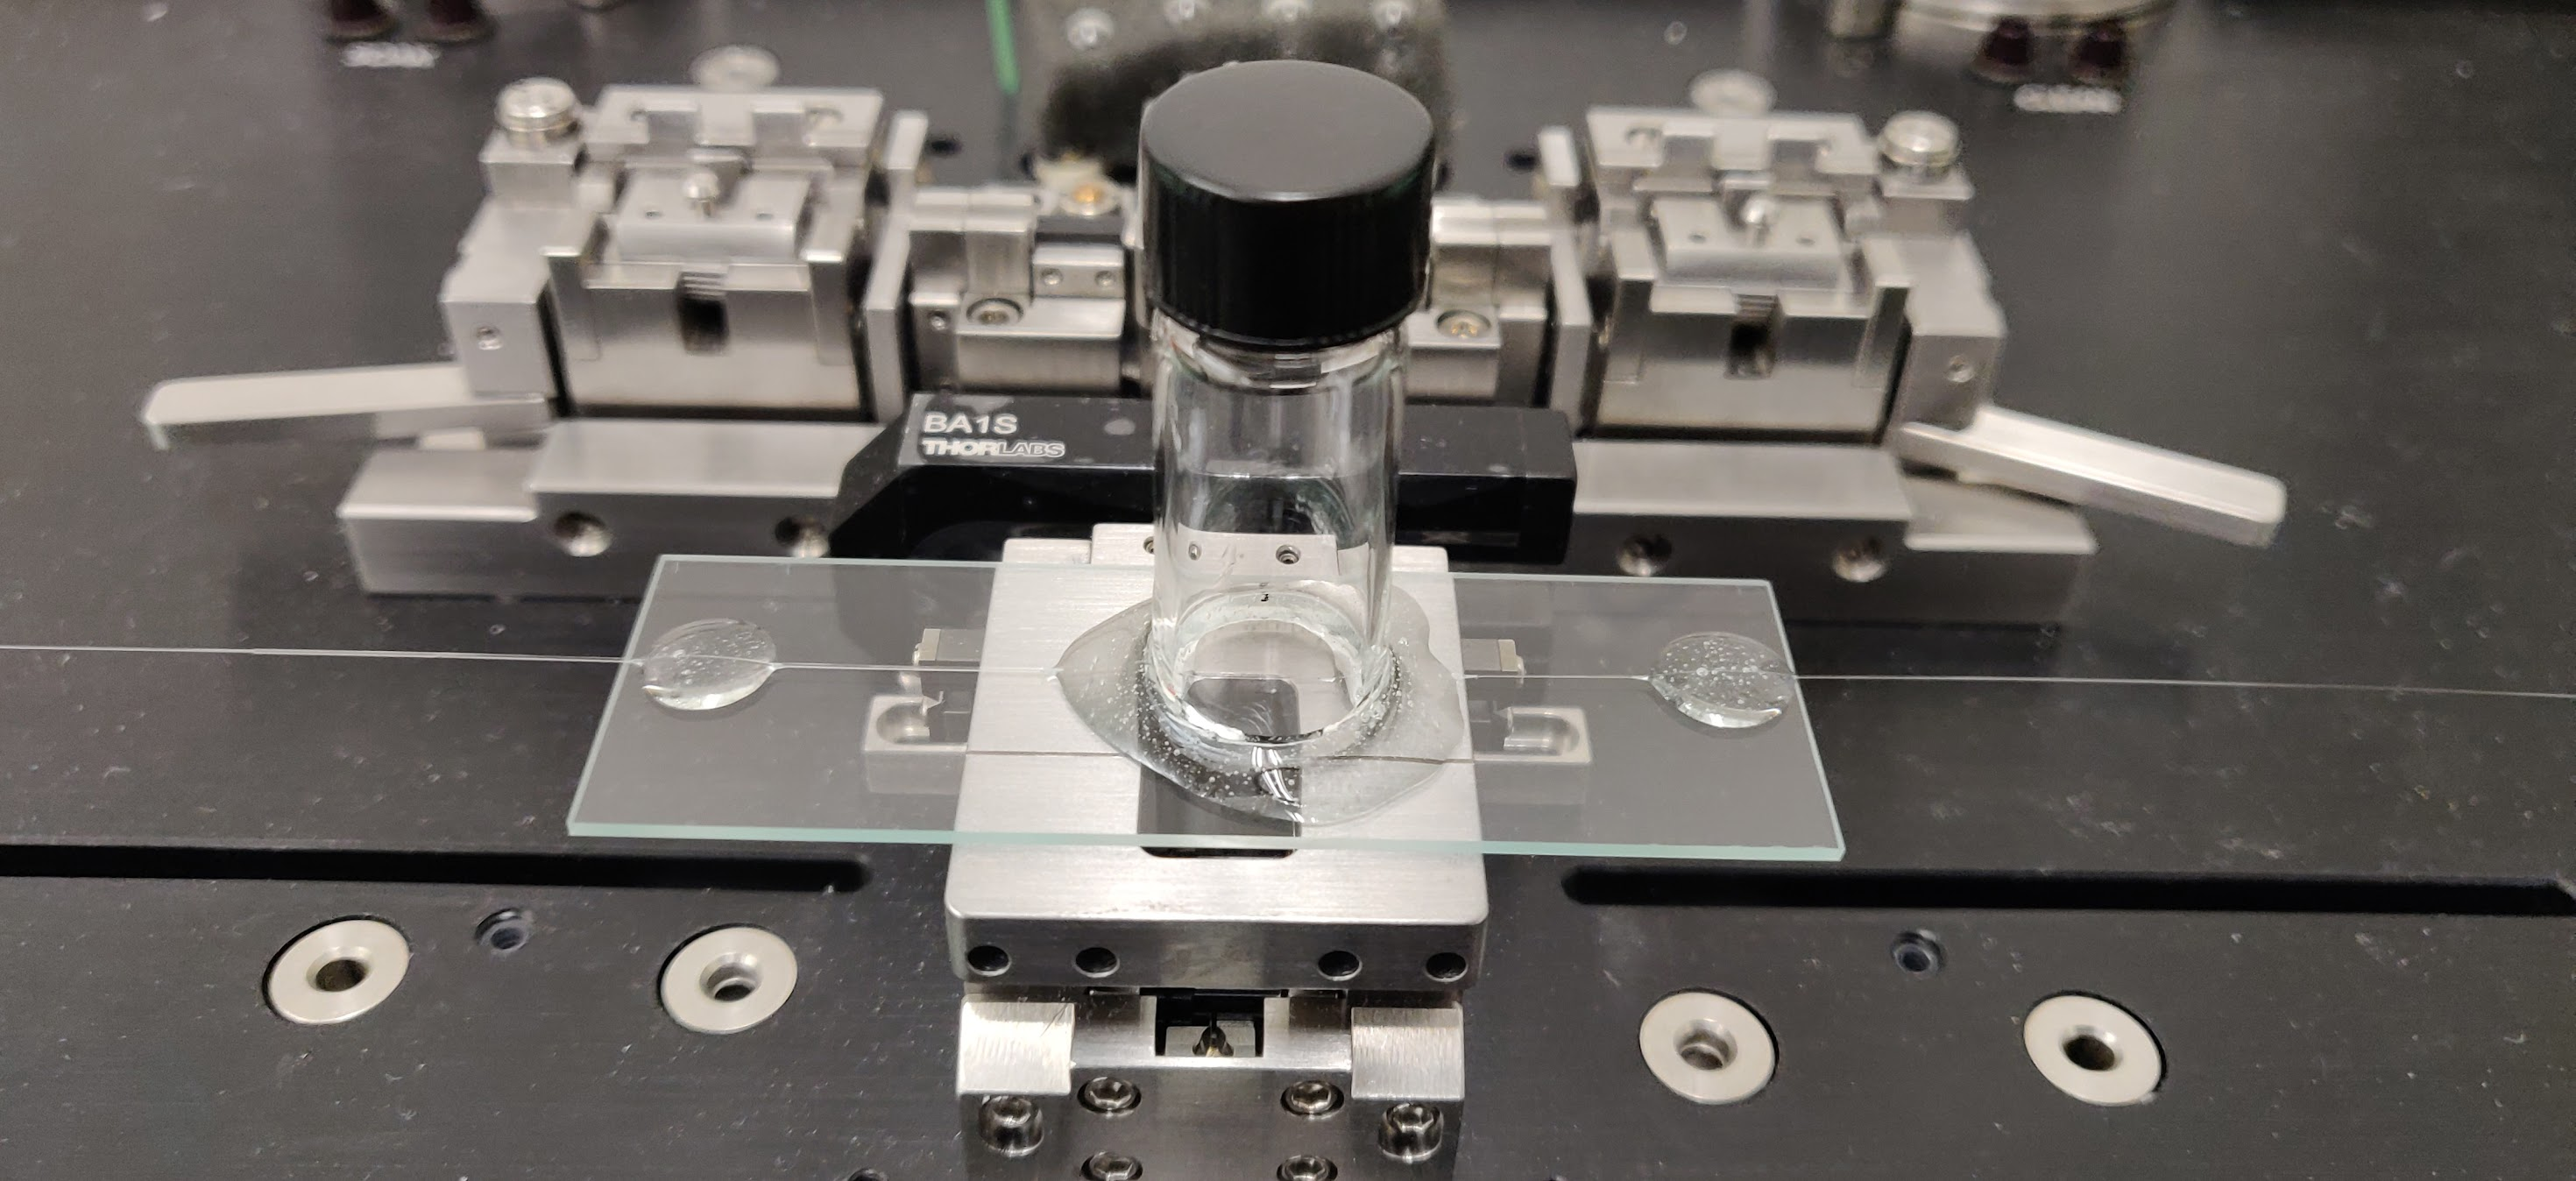
\includegraphics[width=\textwidth]{figs/3-Cooling/successfullyBuiltSplice.jpg}
  \caption{Picture of a complete splice assembly (Section~\ref{subsec:Cooling:Enclosing the Splice}). The hardened epoxy around the base of the vial securely holds the cut and notched vial onto the slide, forming a sealed reservoire around the critical splice. The reservoire is later filled with liquid \ce{CS2} by easy removal of the screw-off cap in order to submerge the critical splice and begin the filling process of the hollow-core fiber via capilary action.}
  \label{fig:successfully build splice}
\end{figure}

\subsection{Enclosing the Splice with the Cut Vial}
\label{subsec:Cooling:Enclosing the Splice}

The splice region was enclosed in a glass vial to protect the hollow-core’s interior and to facilitate later filling with liquid:

\begin{enumerate}
	\item Positioning the Vial: The prepared vial was placed over the splice region by sliding one straddle-gap around the fiber first, then tilting it so the second gap aligned. Gloves were worn to prevent transferring skin oils onto the vial.
	\item Epoxy Sealing: A fresh mixture of two-part epoxy was prepared in roughly equal proportions and thoroughly mixed for 10–15 seconds to ensure a uniform bond. Generous epoxy was applied around the vial’s perimeter where it contacted the slide. Care was taken to avoid epoxy wicking into the splice itself. The assembly was then left undisturbed for at least five minutes to cure.
\end{enumerate}

\begin{figure}[t]
  \centering
  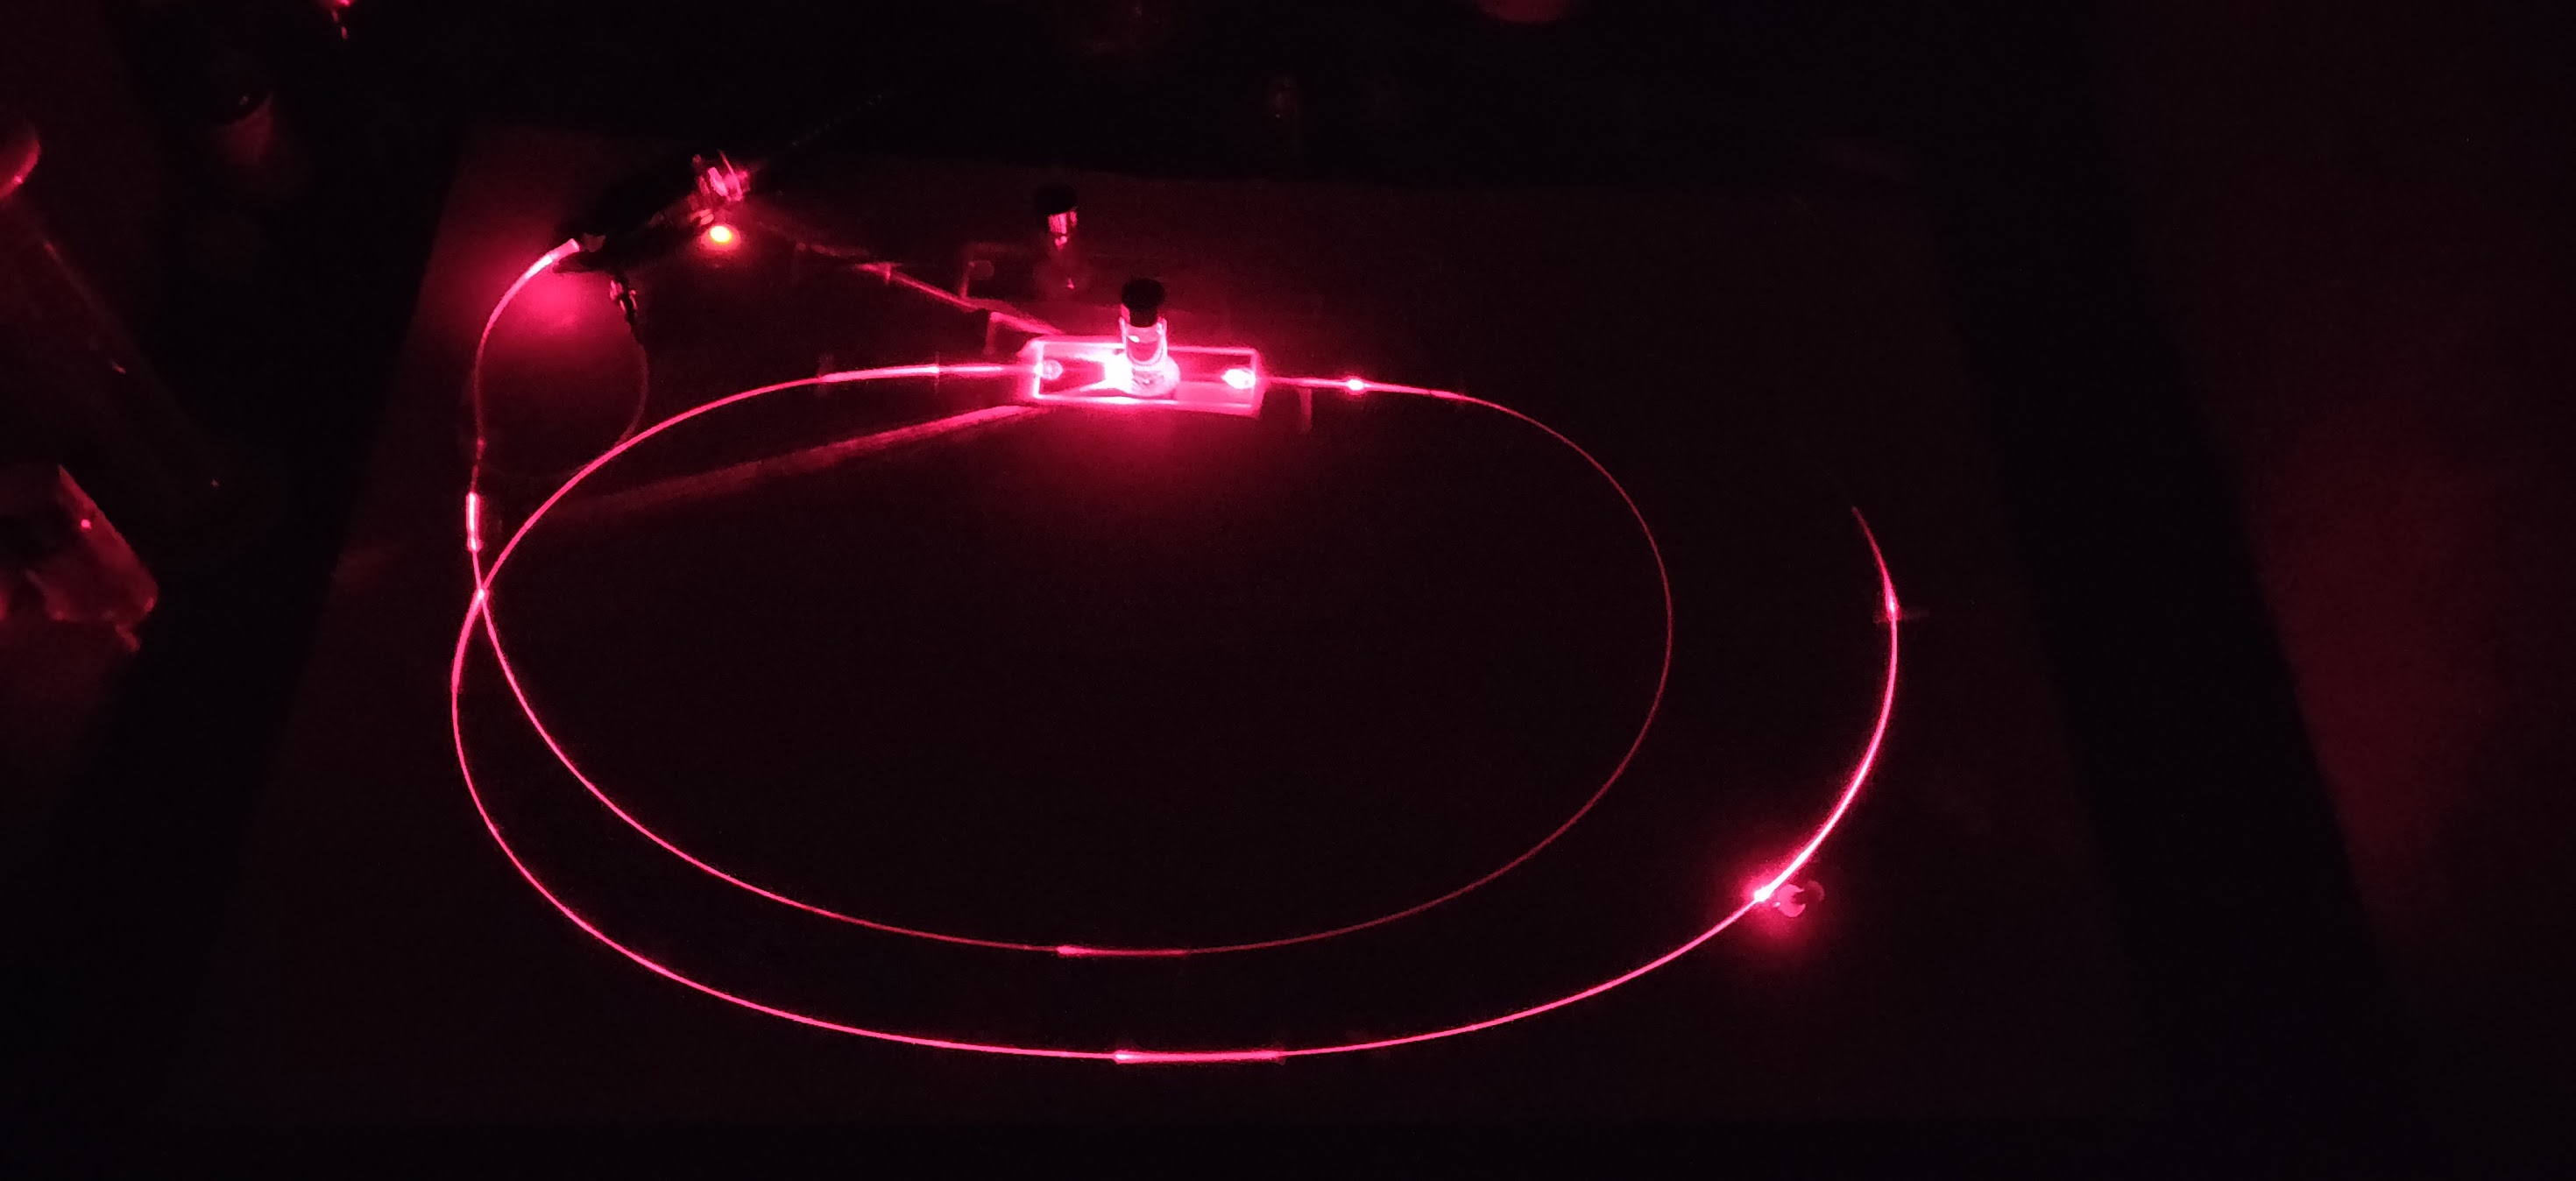
\includegraphics[width=\textwidth]{figs/3-Cooling/redLightWithThumbTackWholeSample.jpg}
  \caption{Picture of a complete sample under the fume hood with lights dimmed and red laser light injected into the end of the sample for monitoring (Section~\ref{subsec:Cooling:Filling with CS2}). The red light is partially guided along the length of fiber which has filled with liquid \ce{CS2} and a thumb tack marks the progress of the \ce{CS2}-air interface.}
  \label{fig:red Light with Thumb Tack Whole Sample}
\end{figure}

\subsection{Final Mounting and Labeling}

Once the epoxy had set, the slide was labeled with the date, splice reference, and relevant notes using a marker. For long-term handling, the slide and its fibers were taped to a foam board or a similarly stable surface to prevent accidental jostling. This procedure ensured a robust, low-loss transition from \ac{SMF-28} to \ac{UHNA7} to the hollow-core fiber. The careful cleaning steps, controlled splicing environment with argon shielding, and meticulous handling minimized the risk of fiber breakage and guaranteed a clean optical interface. Encapsulating the splice with a modified glass vial on a microscope slide allowed easy manipulation of the hollow core’s environment, which was crucial for subsequent liquid filling and optical characterization experiments.

Finally, this entire procedure must be repeated on the opposite side of the hollow-core fiber to complete the \ac{LCOF} assembly. Each splice should be robust enough to guide light but also “broken” sufficiently to allow \ce{CS2} to enter the hollow core via capillary action in the next step.

\begin{figure}[t]
    \centering
    \begin{subfigure}[b]{0.49\textwidth}
        \centering
        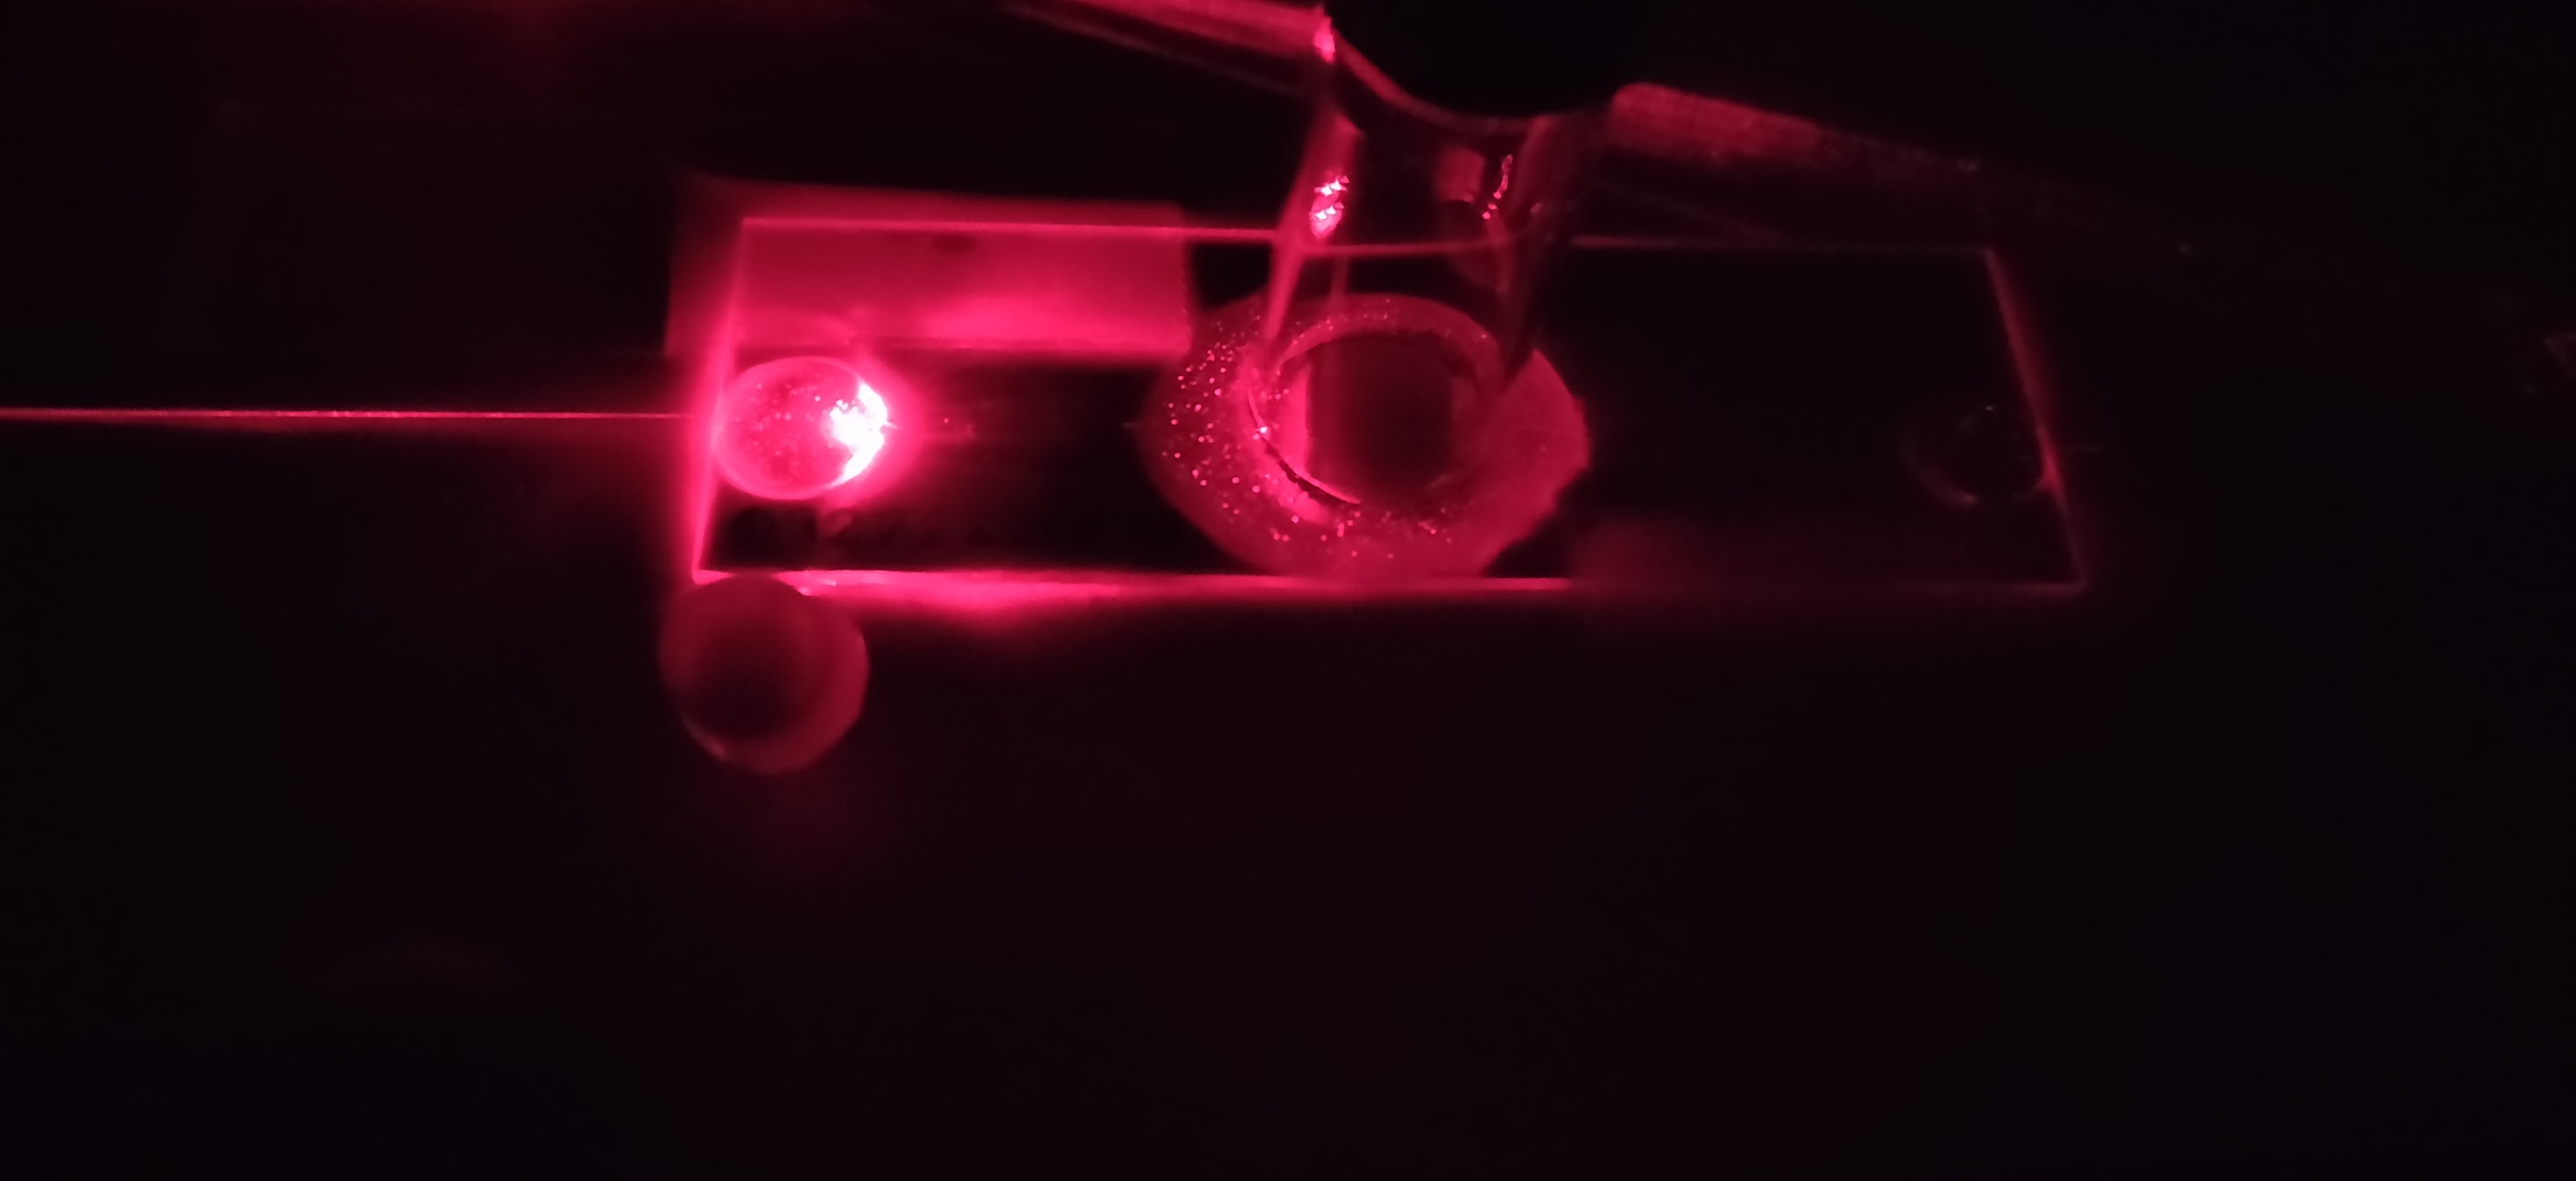
\includegraphics[width=\textwidth]{figs/3-Cooling/CS2NearlyReached.jpg}
        \caption{}
        \label{fig:Cooling:CS2 Nearly Reached}
    \end{subfigure}
    \hfill
    \begin{subfigure}[b]{0.49\textwidth}
        \centering
        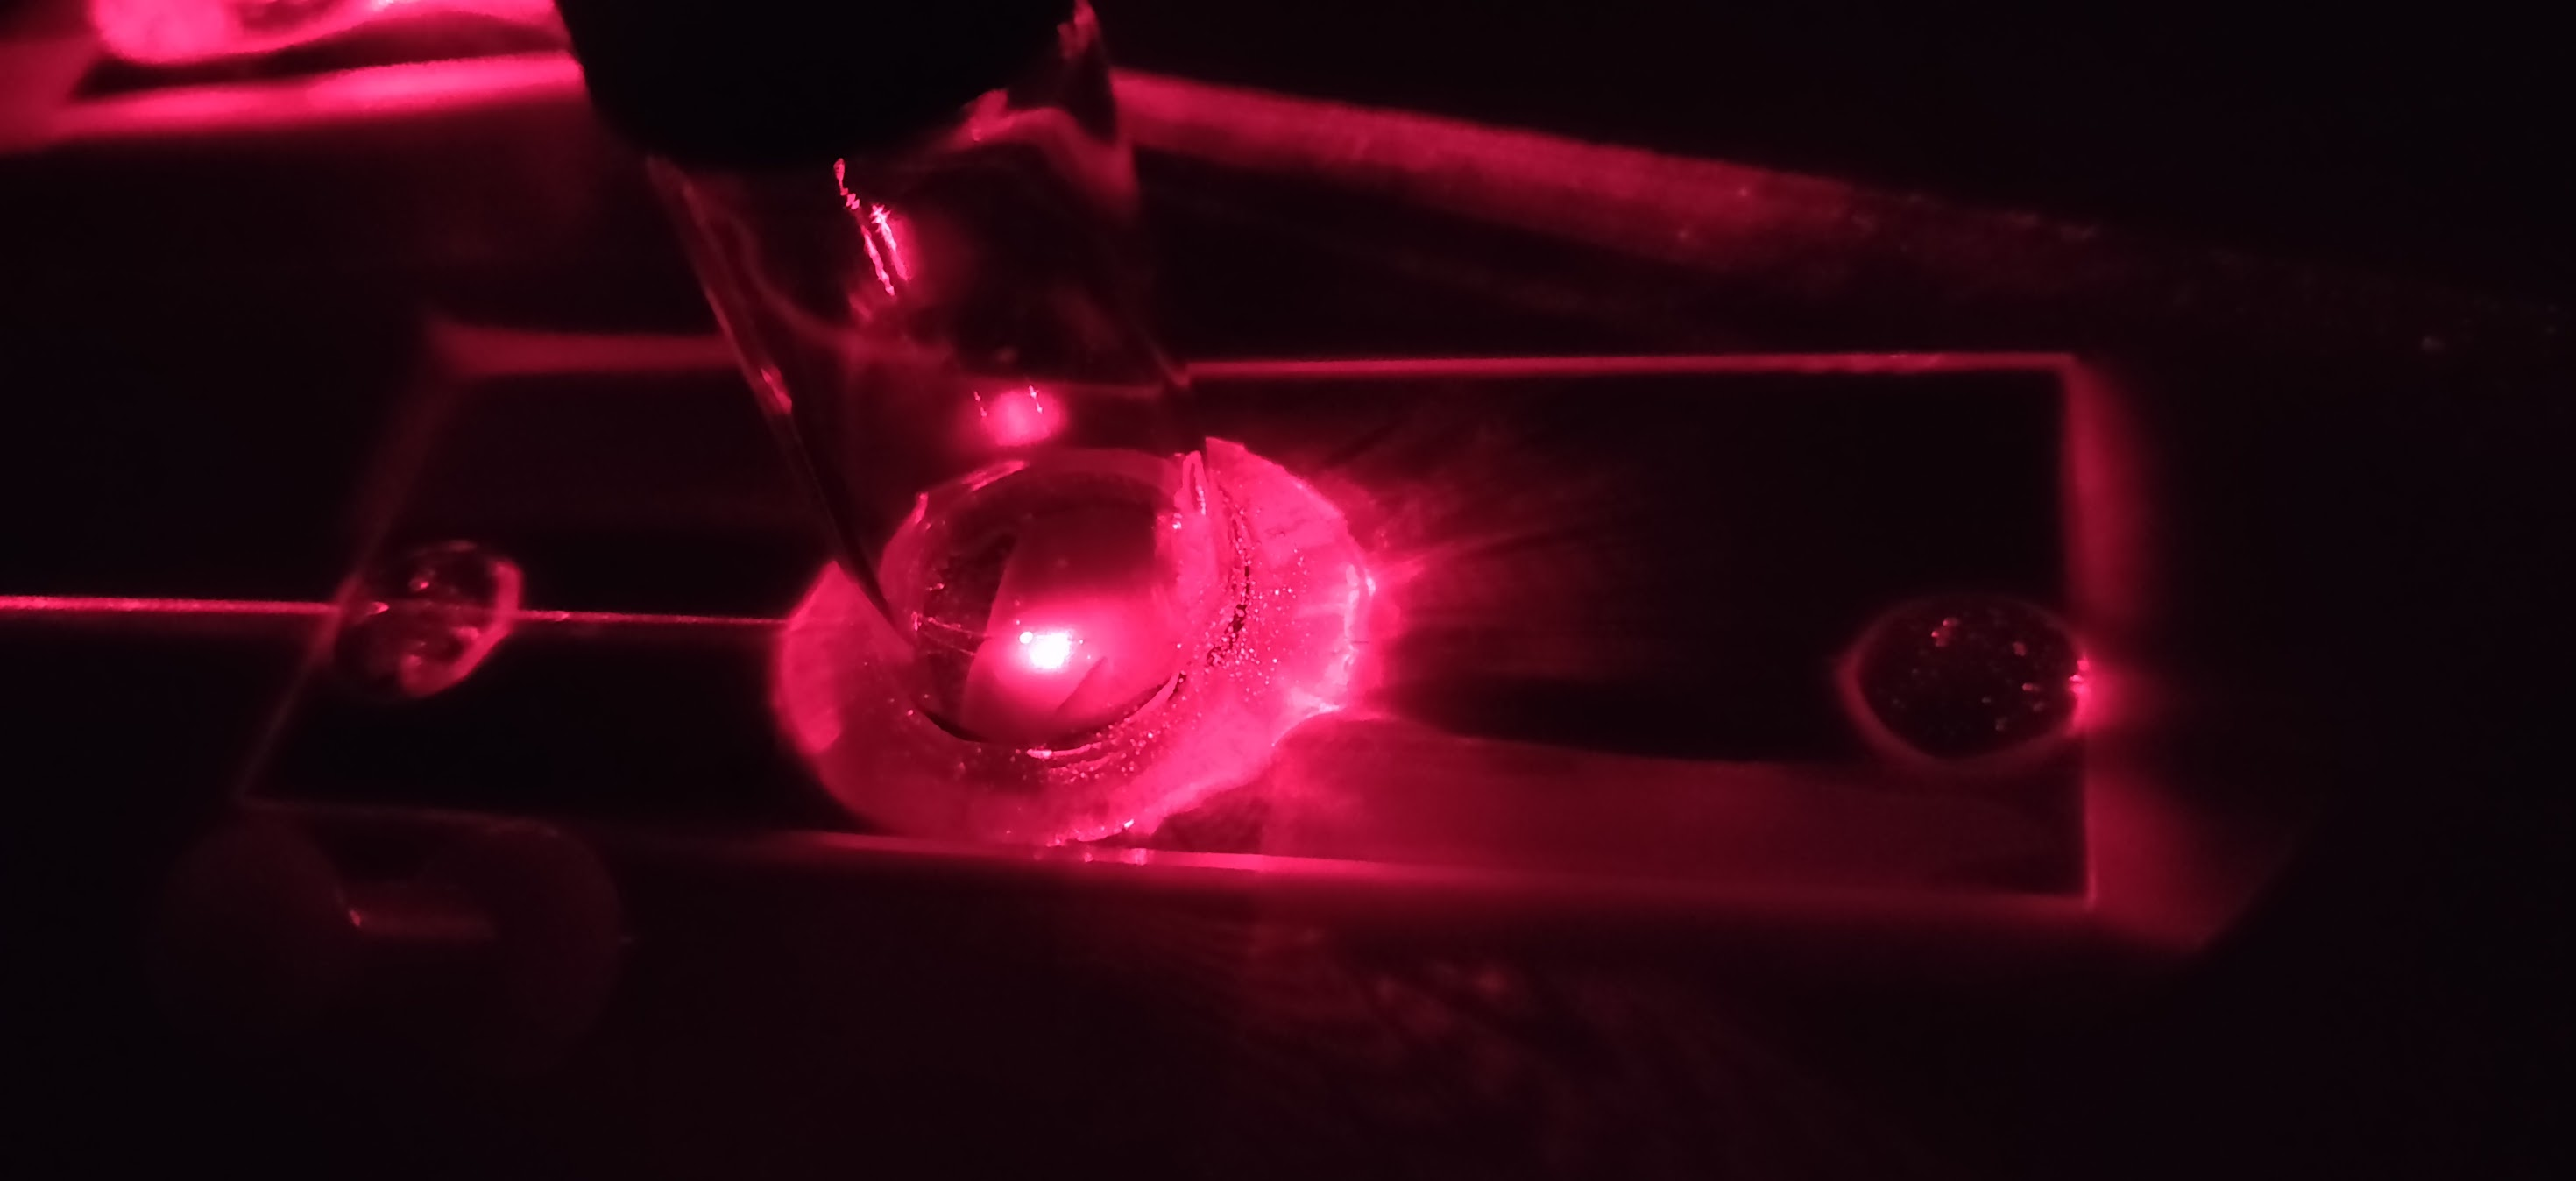
\includegraphics[width=\textwidth]{figs/3-Cooling/CS2Reached.jpg}
        \caption{}
        \label{fig:Cooling:CS2 Reached}
    \end{subfigure}
    \caption{Images of an \ac{LCOF} sample in the filling process (Section~\ref{subsec:Cooling:Filling with CS2}). Figure (a) shows the \ce{CS2}-air interface a few centimeters from the end of the length hollow-core fiber, indicated by the red dot of scattered light just underneath the epoxy tack. From this position, the meniscus will typically reach the exit splice in approximately 4 hours. Figure (b) shows evidence of a fully-filled \ac{LCOF} sample, indicated by the red dot of scattered light having reached the exit splice. If the pictured reservoire were to be filled prematurely, an air bubble would be locked in, reducing full transmission through the sample to nearly 0\%.}
    \label{fig:Cooling:red dot monitoring near the end}
\end{figure}

\subsection{Filling the \ac{LCOF} with Carbon Disulfide}
\label{subsec:Cooling:Filling with CS2}

Once both ends of the hollow-core fiber were successfully spliced to their respective fiber pigtails, the next critical step involved filling the hollow core with carbon disulfide. Because \ce{CS2} is highly volatile and poses health risks if inhaled, all operations were carried out in a fume hood with proper protective equipment.

The prepared \ac{LCOF} sample, securely taped to a poster board, was transferred to the fume hood. A small red laser source was connected to the input pigtail; this red beam served as an in situ indicator of the fluid-filling front. The vial on the input side was uncapped, and the vial on the opposite side was loosened to prevent pressure buildup within the fiber. This arrangement ensured that as \ce{CS2} entered the hollow core, displaced air could escape through the opposite vial, allowing continuous capillary flow.

\subsection{Filling Procedure}

To deliver the \ce{CS2}, a syringe was first used to extract an adequate volume from a sealed supply bottle. The needle tip was then removed and replaced with a micron-level particulate filter, thereby minimizing the introduction of debris that could obstruct the hollow core. By gently angling the syringe, \ce{CS2} was dispensed along the interior wall of the vial rather than dripping directly onto the delicate splice region. This careful approach reduced mechanical shocks, which could otherwise fracture or misalign the newly formed splice. Once the vial was filled, it was recapped promptly to prevent evaporation.

If a given splice was imperfect—fully sealed at the fiber core rather than partially open—it prevented \ce{CS2} from flowing in. Under these circumstances, no visible progression of the fluid meniscus would appear in the red laser beam path, confirming an unsuccessful splice. In contrast, if the splice was partially open, capillary action would begin immediately, typically drawing \ce{CS2} several centimeters into the hollow core within seconds. The interface between the \ce{CS2} and the air still occupying the rest of the fiber showed up as a faintly scattering “dot” in the path of the red beam. By darkening the room, this dot could be easily observed and tracked. Once the fiber was fully filled, the second vial was also filled with filtered \ce{CS2}, then capped. If the second reservoir was filled prematurely, an air bubble would be trapped in the final short length of hollow-core fiber and the resulting transmission through the full length of the \ac{LCOF} would be reduced to nearly 0\%.

Figure~\ref{fig:red Light with Thumb Tack Whole Sample} shows a picture of a sample in the process of filling with \ce{CS2}. Progress is marked by a thumbtack next to the \ce{CS2}-air interface. With the lights turned off, the dot of scattered light at this interface was a reliable visible indicator. Figures~\ref{fig:Cooling:CS2 Nearly Reached} and \ref{fig:Cooling:CS2 Reached} show images of a sample that has nearly finished and fully finished filling, respectively. The filling state captured by Figure~\ref{fig:Cooling:CS2 Nearly Reached} indicates a likely time to finish filling of approximately 4 hours.

\begin{figure}[t]
    \centering
    \begin{subfigure}[b]{0.49\textwidth}
        \centering
        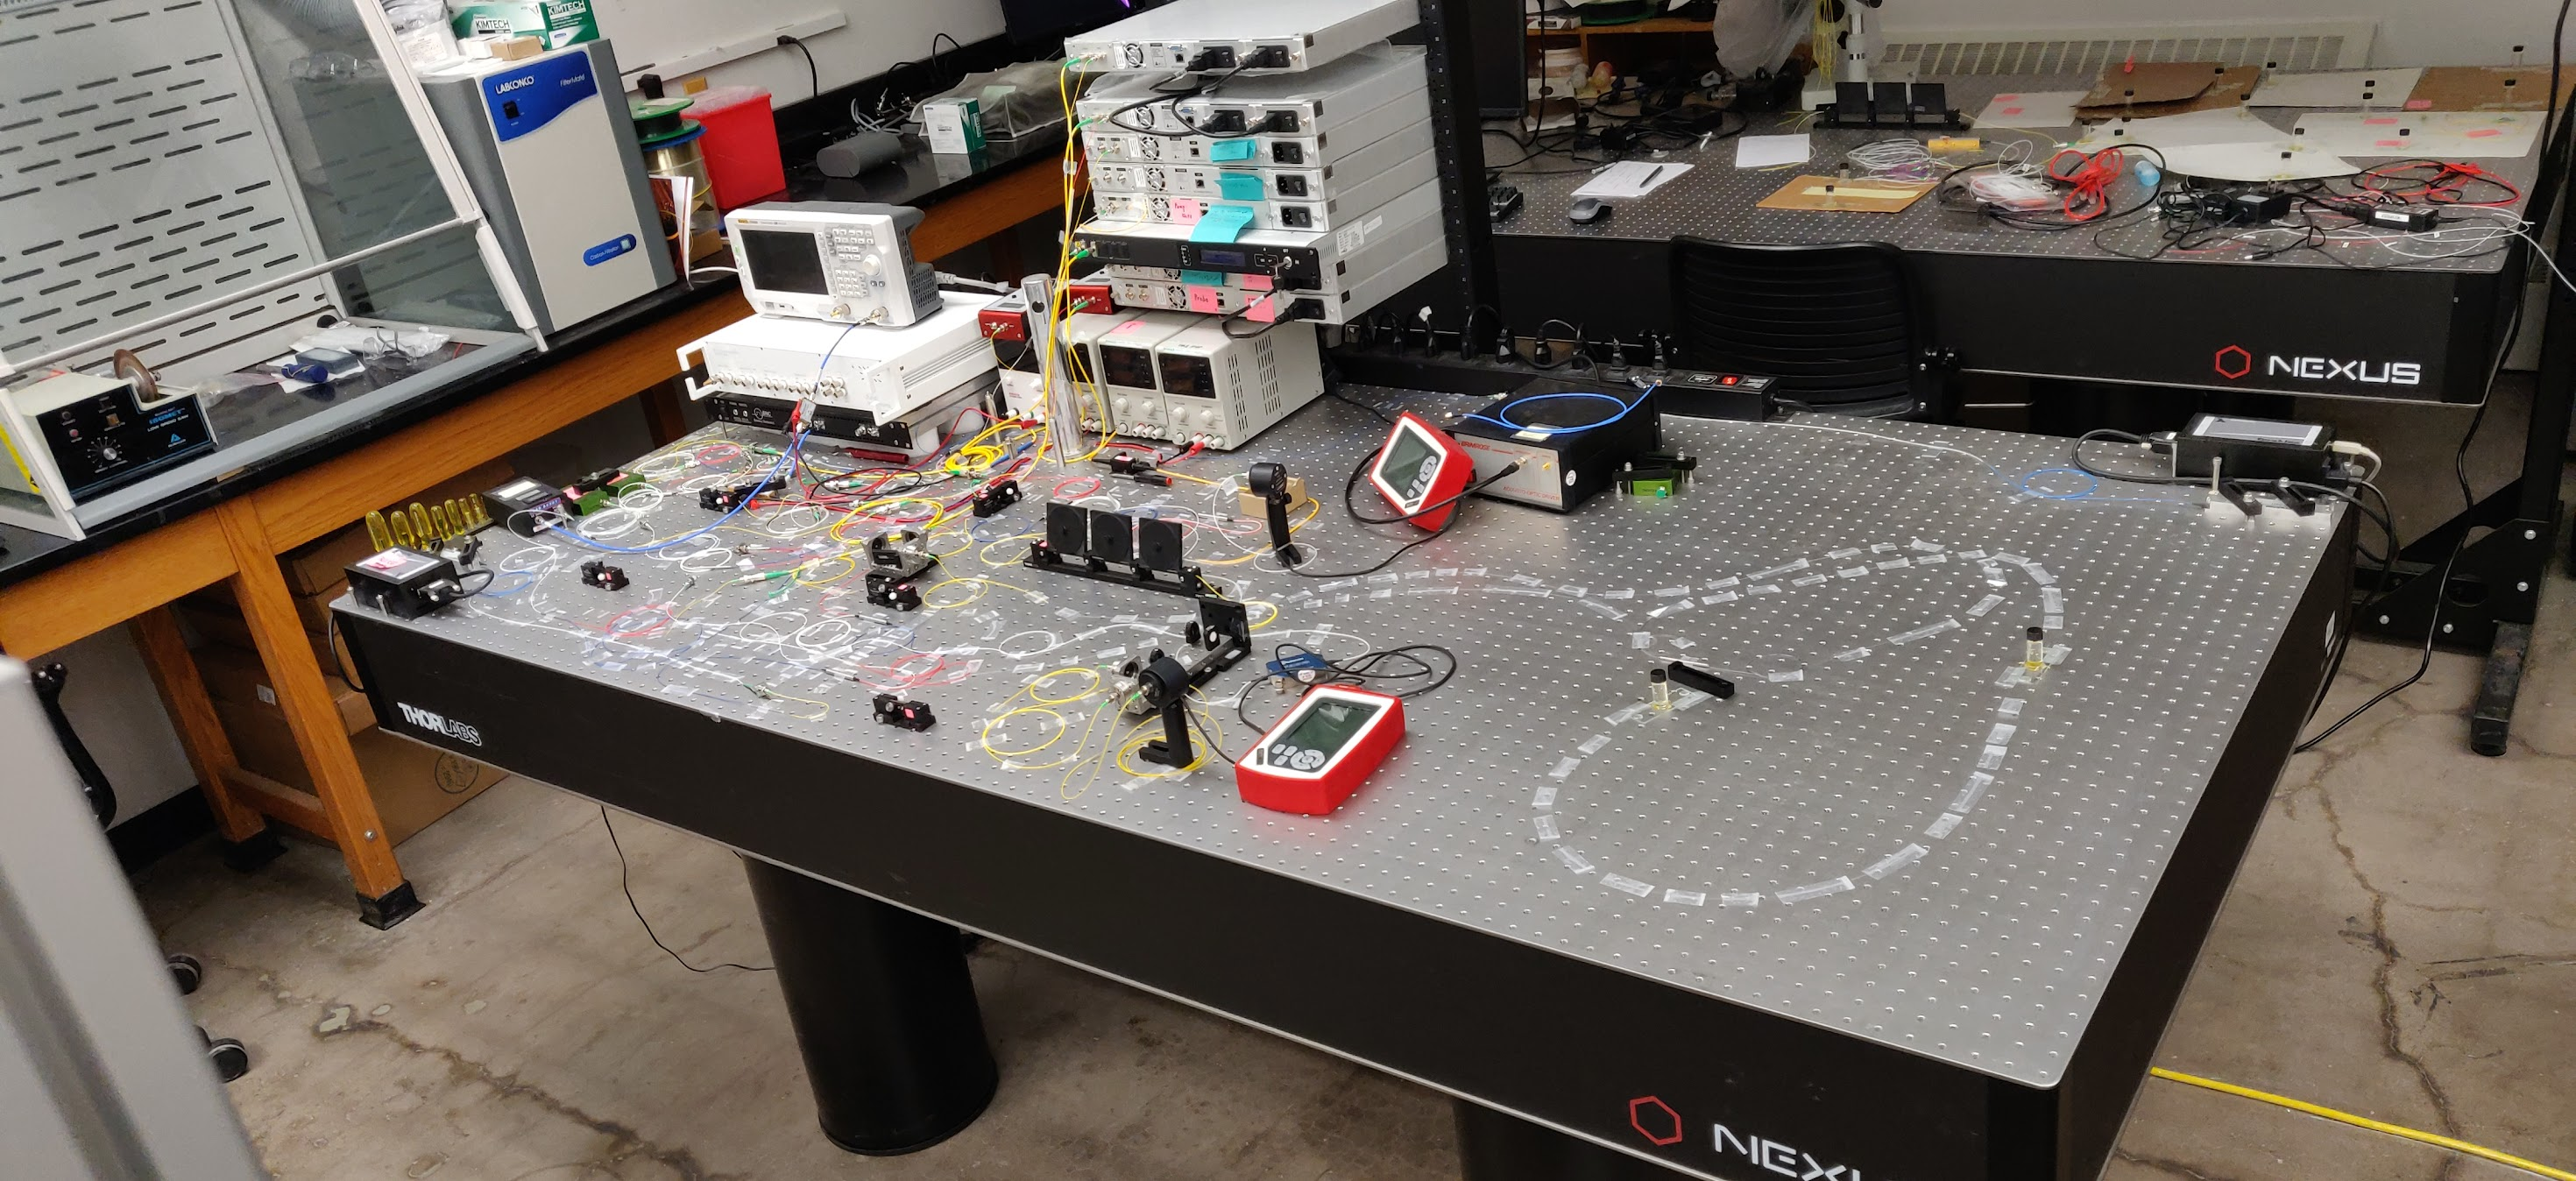
\includegraphics[width=\textwidth]{figs/3-Cooling/fullSampleTapedToOpticalTable.jpg}
        \caption{}
        \label{fig:Cooling:Full Sample Taped on Table}
    \end{subfigure}
    \hfill
    \begin{subfigure}[b]{0.49\textwidth}
        \centering
        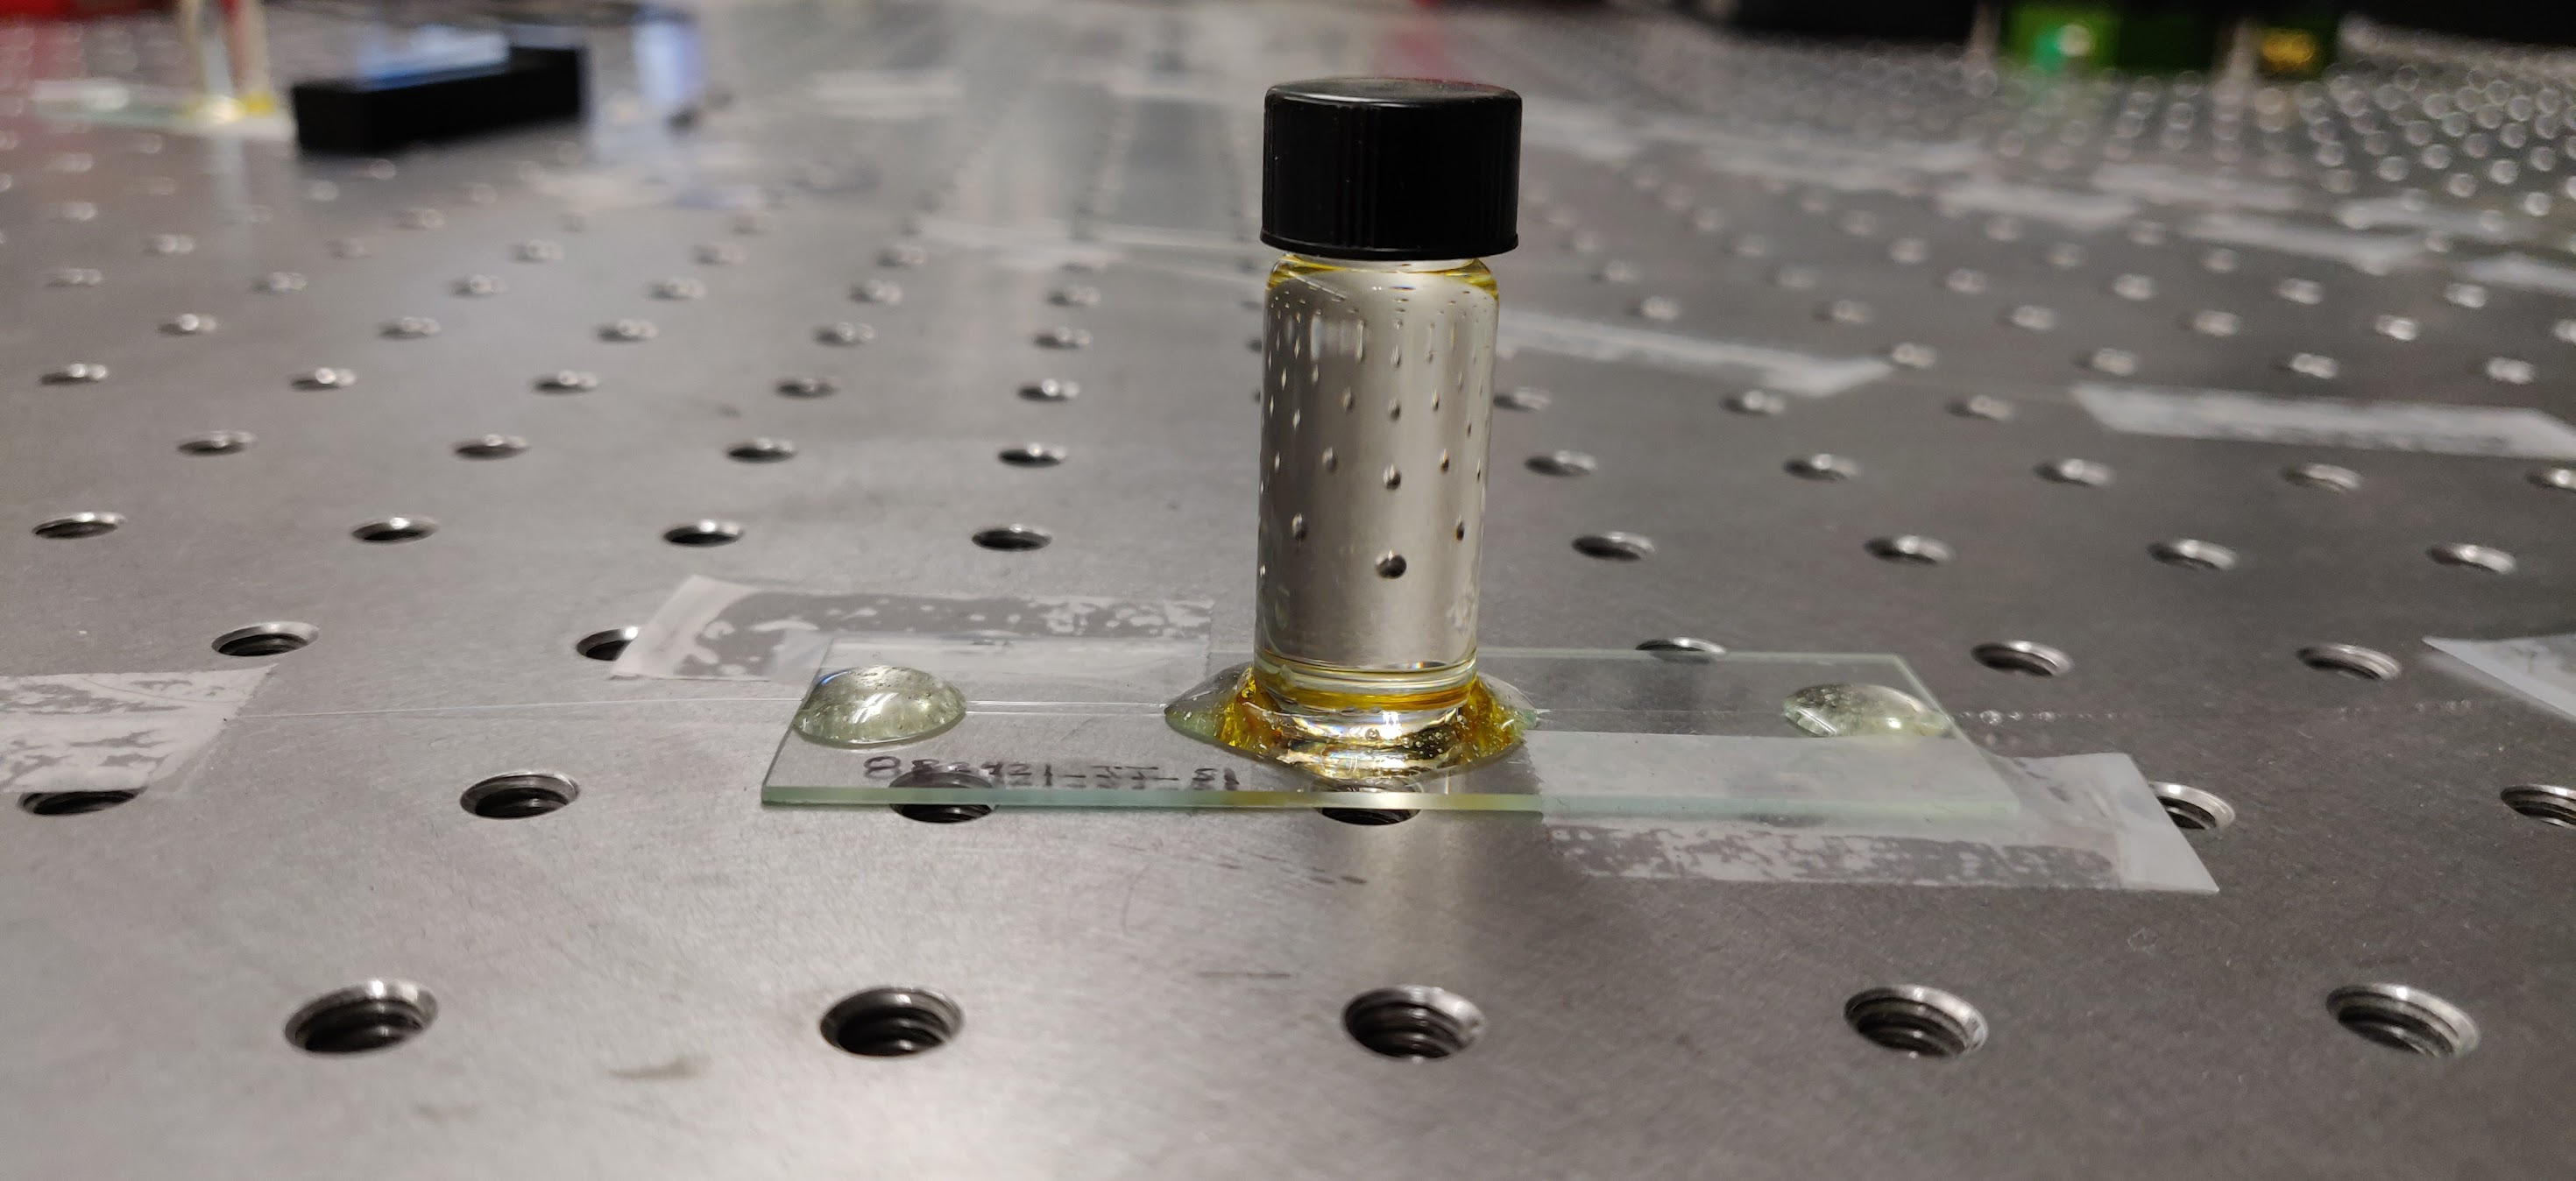
\includegraphics[width=\textwidth]{figs/3-Cooling/spliceTapedDirectlyOnOpticalTable.jpg}
        \caption{}
        \label{fig:Cooling:Splice Taped on Table}
    \end{subfigure}
    \caption{Images of a fully finished \ce{CS2}-\ac{LCOF} sample (Section~\ref{subsec:Cooling:Typical Optical Performance}). Figure (a) shows a sample secured with tape to an optical table and integrated into an optical setup. Liberal use of tape ensured the safety of the sample as well as reduced vibrations and minimized changes in the polarization of light travelling through the sample. Figure (b) shows one splice assembly secured directly to the optical table via tape. Transfer of all parts of the sample from the poster board directly onto the optical table proved critical for eliminating noise and polarization drift issues with the pump-probe experiment.}
    \label{fig:Cooling:LCOF Taped on Table}
\end{figure}

\subsection{Typical Optical Performance}
\label{subsec:Cooling:Typical Optical Performance}

Optical transmission at each splice typically ranged from 15–30\%. However, the final \ac{LCOF} used in the published experimental demonstrations achieved full throughput transmission of about 54\%. This suggests each splice individually could guide on average approximately 75\% of the incident light when accounting for the back-and-forth path of the Brillouin scattering measurements. For demonstration of optomechanical cooling of traveling-wave phonons in this \ac{LCOF}, the ability to maintain a stable liquid-core environment was crucial, and the patient filling protocol proved instrumental in obtaining reliable backscattering results.

This stepwise filling method, combined with patient observation, thorough cleaning, and meticulous splicing, yielded reproducibly filled fibers that supported the subsequent optical and optomechanical experiments. By overcoming prior misconceptions about the time needed for complete filling, the protocol minimized fiber waste, saved costs, and ensured that each sample was thoroughly filled and ready for precise measurements.

\subsection{Maintaining the Filled Sample}

Over periods of days, some evaporation was inevitable; replenishing the vials every two to three days extended the operational lifetime of the sample. Despite occasional epoxy degradation at the splice site, which might reduce forward transmission, the backscattering experiments remained unaffected except for a loss of forward transmission monitoring. In most cases, even months-long sample preservation and continued experimentation was feasible with proper maintenance.

\subsection{Innovations in Yield and Performance of \ac{LCOF} Samples}

A key refinement that greatly improved sample fabrication success rates was the adoption of extremely careful post-splice handling. Previously, standard procedure was to lift the newly spliced fiber assembly without ensuring that each side was completely free of the splicer’s grooves. This led to abrupt bending or sudden “snapping” out of the clamp grooves, which almost invariably broke delicate splices that were only partially fused. The implementation of several measures helped to avoid this failure mode. First, folded-paper “sawhorses” and two small Kimwipe boxes on each side of the splice were placed to support the fibers and reduce vibration or flexing. Before switching off the vacuum seal, the clamp latches were gently lifted and small wooden sticks were used to ease the fibers out of the translation/rotation block grooves, ensuring there was no latent twisting or bending. Throughout these steps, the fibers were kept as close as possible to their natural resting position, minimizing stress that would be transferred to the just-completed splice. This careful approach not only reduced the chance of breakage but also allowed for the feasibility of splices that remained sufficiently “open” for \ce{CS2} to enter the hollow core, substantially increasing the proportion of successfully filled samples.

In using the slow-rotation saw to cut and form notches in the glass vial, simple improvements in notch geometry greatly reduced breakage of splices while placing the vial on the slide overtop the delicate splice, and straddling the fibers on either side. Cutting notches to be \(\sim\SI{1}{\centi\meter}\) (10-20 times the width of the fiber) reduced the risk of inadvertently contacting the fibers and breaking the delicate splice during vial placement. Additionally, cutting the notches to be shallow (approximately 5 times the width of the fiber) prevented epoxy from running through the notch and sealing the splice. Previous standard procedure were opposite to this geometry as a natural result of the narrow width of the saw blade and the depth to which it could easily be allowed to cut.

A key innovation in the filling procedure was performing a long observation of the filling process for one sample. Previous standard procedure was to stop monitoring after 8 or 12 hours, assuming the fill process had ceased or completed but subsequently reversed if the fluid had not reached the far end by that time. Through extended trials, it was discovered that in successful splices, the fill front progresses at a nonlinear, steadily decreasing rate, and that a one-meter fiber segment migh take more than 24 hours to completely fill. In one particularly instructive case, continuous monitoring for 27 hours without leaving the room as a sample filled confirmed that the \ce{CS2} front never reversed; it merely advanced extremely slowly in the final length to reach the other end. Alarms were set for inspection every 90 minutes throughout the night in the final hours of monitoring the sample under the fume hood. Having observed and documented this behavior, the standard practice became allowing the sample to sit undisturbed for at least a full day or more, ensuring the fiber was completely saturated before concluding success or failure. This observation effort and resulting insight halted the regular production of significant waste of both material and time in the fabrication process of \ac{LCOF} samples.

A final insight that improved the yield of successfully filled samples and mitigation of wasted materials was selecting the “less certain” end of a prepared sample for filling with \ce{CS2}. If that splice was sealed, only that end would need to be re-fabricated. Collectively, these simple method improvements in sample fabrication led to significantly shorter fabrication times and dramatically reduced material waste. Hollow-core fibers, which cost on the order of ten dollar per meter, were previously scrapped in large quantities when deemed “dead.” By implementing patient monitoring, careful handling, and mindful filling procedures each length of fiber was used more efficiently, saving significant time and expense while producing more effective samples.

%--------------------------------------------------------------------%

\section{Experimental Setup}
\label{sec:Cooling:Setup}


\subsection{Main Experiment}
\label{subsec:Cooling:Setup:Main}


\subsection{Pump-Probe Experiment}
\label{subsec:Cooling:Setup:Pump-Probe}

%--------------------------------------------------------------------%

\section{Results}
\label{sec:Cooling:Results}


\subsection{Main Experiment Results}
\label{subsec:Cooling:Results:Main}

need for normalized cooling metric - per pump power, and such that one cannot start a system in a heated state to achieve a greater stated cooling ability. Or maybe room temperature is identical across systems? check. if not, normalize.

\subsection{Pump-Probe Experiment Results}
\label{subsec:Cooling:Results:Pump-Probe}

%--------------------------------------------------------------------%

\section{Discussion}
\label{sec:Cooling:Discussion}

Ideas to achieve net cooling, one might design a system where:

1) single pass gain bias
     swing energy transfer bias to favor anti-Stokes over Stokes (mode-dependent gain)
     the Stokes process were not permitted (ryan's only idea), or just significantly restricted - what is that bias threshold requirement?
     currently, we are net *heating* the system because it is easier to heat from equilibrium than cool (right? explore this. it's also hard to make it hotter beyond a certain point.)
     implementation ideas:
       multi-pump scheme to destructively interfere with Stokes and/or constructively interfere with anti-Stokes
       doping or specialized waveguide gratings that pick out the Stokes band for out-of-plane scattering

2) time bias
     create an energy transfer *rate* bias between Stokes and anti-Stokes
     can be accomplished with either the brillouin energy transfer rate or the repopulation rate

       brillouin process rate:
         4vg/L, have either group velocity or length be different for Stokes vs anti-Stokes (smaller vg or larger L for Stokes than anti-Stokes)
         make anti-Stokes fast light and/or Stokes slow light
         vg inversely proportional to pump power, so it's a balance
           increasing pump power = slower escape time (4vgL), and also larger dissipation (Gamma+)

       repopulation rate:
         thermally insulate the anti-Stokes mode from the thermal bath that would repopulate it
         or at least insulate it some amount more than Stokes (what is that threshold? even if it's only net cooled for picoseconds, what is that minimum crossover point insulation bias point)
         essentially locks in the cooled mode while letting the heated mode spill out
         implementation idea:
           design a fiber/waveguide with acoustic directional bias, such that phonons travelling one direction dissipate quicker because of the geometry/acoustic properties of the fiber. (triangles? acting as tapered acoustic dissipators, pointing in one direction?)

3) starting temperature
     Could you acieve net cooling in a cheap and dirty sense by starting the system in a very heated state, thus invoking a natural dissipation rate bias?! - yes!
     Things do naturally run hot, perhaps no extra fancy engineering is needed for some practical systems? (data processing, reduce thermal noise from above ambient heat)
     not traditional definition of optical refrigeration below ambient/thermal bath, but still *useful*
     is this already done? lit search

Think about a practical device or system for each of these cases (think waveguide playground!)

\subsection{Application to Ground State Cooling}
\label{subsec:Cooling:Discussion:Ground-State}


\subsection{Standardized Cooling Metric}
\label{subsec:Cooling:Discussion:Metric}


\subsection{Tapered chalcogenide Photonic Crystal Fiber: Max Plank Results}
\label{subsec:Cooling:Discussion:Max-Plank}
